

\documentclass[apuntes]{uc3mmaster}

\titulo{Aprendizaje evolutivo de la representación de los datos para modelos basados en distancias}\asignatura{IA con inspiración biológica.}\tipo{Apuntes}
\autor{Andrea López Salazar}{}
\usepackage[utf8]{inputenc}
\usepackage[T1]{fontenc}
\usepackage{graphicx}


% ---- Paquetes para las figuras ----
\usepackage{tikz}
\usetikzlibrary{babel}
\usepackage{pgfplots}
\pgfplotsset{compat=1.18}
\usetikzlibrary{arrows.meta, positioning, calc, shapes.geometric, decorations.pathreplacing}
\usepackage{booktabs}

% Si usas babel en español, evita conflictos con las flechas de TikZ:
% \usepackage[spanish, es-noshorthands]{babel}
% (o bien añade la librería: \usetikzlibrary{babel})

% ---- Colores ----
\definecolor{azul}{HTML}{2E5EAA}
\definecolor{naranja}{HTML}{E07A1F}
\definecolor{verde}{HTML}{3A8F5C}
\definecolor{rojo}{HTML}{C0392B}
\definecolor{gris}{HTML}{8C8C8C}
\begin{document}
\makeportada
\section{Problema}
Nos piden un programa P que, dado un conjunto de entrenamiento $(X_t, y_t)$, aprenda con técnicas de computación evolutiva una transformación del los atributos: síntesis de atributos o reducción de dimensionalidad. Esa transformación se aplica después al conjunto de validación: $X_v'=v(X_v)$. 

Si entrenamos un modelo arbitrario M con los atributos originales y medimos el error absoluto medio (MAE) en validación, obtenemos \textit{e}. Si entrenamos el mismo m odelo M con los atributos transformados y obtenemos \textit{e'}, el método funciona cuando \textit{e'}<\textit{e}.
\subsection{Planteamiento}
\begin{itemize}
    \item El modelo M es arbitrario. Por eso evaluamos siempre con varios modelos --- regresión lineal, KNN y árbol de decisión --- y no con uno solo. 

    \item La transformación se aprende solo con el entrenamiento, siendo la validación lo único que usamos para medir. 

    \item Buscamos un método generalizable que funcione igual en datasets distintos sin ajustes a mano. 
\end{itemize}

\subsection{Datos}
Partimos de dos datasets de regresión: Diabetes (442 muestras, 10 atributos) y California Housing (20640 muestras, 8 atributos). Para comprobar que el método es generalizable, se usan de manera adicional 10 datasets de OpenML --- la lista y sus tamaños los tenemos en una sección posterior.

\subsection{Protocolo común}
\begin{itemize}
    \item Usamos una partición con 70\% de entrenamiento y 30\% de validación con semillas distintas para cada unas de las repeticiones.

    \item La métrica va a ser el MAE en el conjunto de la validación. 

    \item Para poder comprobar datasets con escalas muy distintas, usamos el MAE relativo a los datos originales, y el MAE/MAE(crudo), promediado con la media geométrica. Si es menor que 1, significa que hemos mejorado. 

    \item Contrastes estadísticos, incluido el test de Wilcoxon por pares, aplicado sobre el cociente de errores de cada pareja (dataset, partición).
\end{itemize}
\newpage
\section{Teoría}
\subsection{Importancia de la representación en KNN (modelos basados en distancias)}
\subsubsection{Predicciones del KNN}
Para poder predecir el valor de un punto nuevo $q$ se bucan los $k$ puntos del entrenamiento más cercanos a $q$, devolviendo la media de sus valores $y$. No construye un modelo, sino que guarda los datos $y$, y en cada consulta mira a los vecinos. 

Todo se apoya en el supuesto de que los puntos cercanos tienen valores parecidos. Por ello la calidad del KNN depende de las distancias. Usualmente, usamos la distancia Euclídea. 

$$ 
d(x, x')^2 = \sum_{j} (x_{j}-x_{j}')^2
$$

Para cada atributo, restamos los dos valores, elevados al cuadrado, y lo sumamos todo. 

\subsubsection{Valor de los atributos}
La fórmula suma las diferencias de todos los atributos con el mismo peso. Parece neutral, pero el resultado depende de las unidades y de la forma de cada atributo. Aquí nos encontramos con tres problemas: 

\begin{enumerate}
    \item \textbf{Escala}: Si un atributo mide en miles y otro en unidades, el primero domina la suma, aunque no sea el más útil. 
    \item \textbf{Atributos irrelevantes}: Cada atributo que no aporta información, añadiendo una diferencia que es puro ruido. Con varios así, la distancia refleja más ese ruido que la similitud real, y muchos de los $k$ vecinos dejan de ser vecinos de verdad. Cuando hay muchas dimensiones, todas las distancias tienden a parecerse y el ''más cercano'' deja de tener sentido. Esta es la maldición de la dimensionalidad. La \autoref{fig:vecindarios} nos muestra cómo cambia el vecindario de un mismo punto según la representación.
    \item \textbf{Distribuciones sesgadas o con valores extremos}: Si unos puntos tienen valores enormes, ocupan casi todo el rango y el resto queda comprimido a una franja estrecha. Incluso estandarizando, las diferencias entre los puntos normales son minúsculas y el atributo apenas distingue donde están la mayoría de datos (\autoref{fig:compresion}).
\end{enumerate}

\begin{figure}[htbp]
\centering
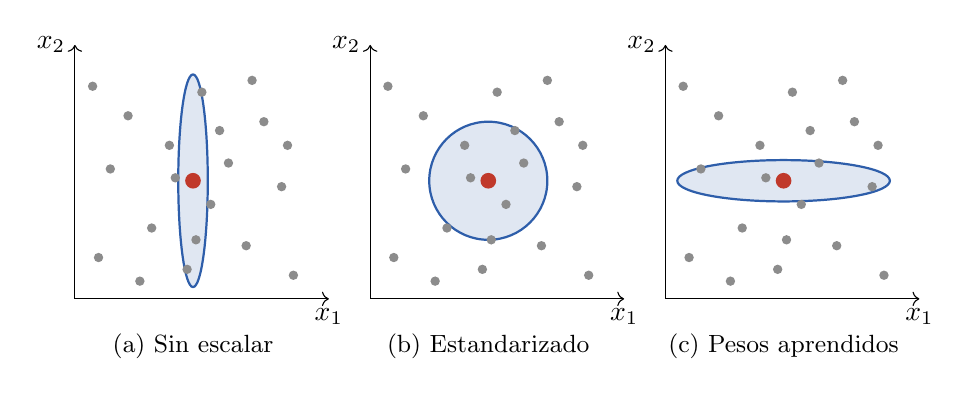
\begin{tikzpicture}[scale=0.75,
  pt/.style={circle, fill=gris, inner sep=1.2pt},
  qq/.style={circle, fill=rojo, inner sep=2pt}]
\foreach \dx/\titulo/\rx/\ry in {0/{(a) Sin escalar}/0.25/1.8,
                                 5/{(b) Estandarizado}/1/1,
                                 10/{(c) Pesos aprendidos}/1.8/0.35}{
  \begin{scope}[xshift=\dx cm]
    \fill[azul!15] (2,2) ellipse ({\rx} and {\ry});
    \draw[azul, thick] (2,2) ellipse ({\rx} and {\ry});
    \draw[->] (0,0) -- (4.3,0) node[below] {$x_1$};
    \draw[->] (0,0) -- (0,4.3) node[left] {$x_2$};
    \foreach \p in {(0.4,0.7),(0.9,3.1),(1.3,1.2),(1.6,2.6),(1.9,0.5),
                    (2.15,3.5),(2.3,1.6),(2.6,2.3),(2.9,0.9),(3.2,3.0),
                    (3.5,1.9),(3.7,0.4),(0.6,2.2),(1.1,0.3),(3.0,3.7),
                    (0.3,3.6),(2.05,1.0),(1.7,2.05),(2.45,2.85),(3.6,2.6)}{
      \node[pt] at \p {};
    }
    \node[qq] at (2,2) {};
    \node at (2,-0.8) {\small \titulo};
  \end{scope}
}
\end{tikzpicture}
\caption{Vecindario del punto $q$ (rojo) según la representación.
(a) Si $x_1$ se mide en miles, una pequeña diferencia en $x_1$ pesa muchísimo:
solo son vecinos los puntos con $x_1$ casi igual, sea cual sea $x_2$.
(b) Tras estandarizar, ambos atributos cuentan igual y el vecindario es un círculo.
(c) Si se aprende que $x_1$ es poco relevante ($w_1$ pequeño), el vecindario se
alarga en esa dirección y los vecinos se eligen sobre todo por $x_2$.}
\label{fig:vecindarios}
\end{figure}

\begin{figure}[htbp]
\centering
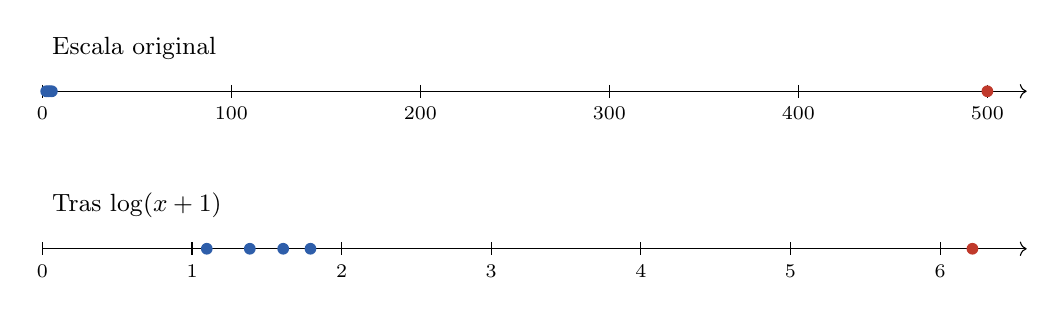
\begin{tikzpicture}[
  pt/.style={circle, fill=azul, inner sep=1.5pt},
  extremo/.style={circle, fill=rojo, inner sep=1.5pt}]
% Escala original: 0..500 -> 0..12 cm
\node[anchor=west, font=\small] at (0,0.55) {Escala original};
\draw[->] (0,0) -- (12.5,0);
\foreach \v in {0,100,200,300,400,500} {
  \draw (\v*0.024,0.08) -- (\v*0.024,-0.08) node[below]{\scriptsize \v};
}
\foreach \v in {2,3,4,5} { \node[pt] at (\v*0.024,0) {}; }
\node[extremo] at (500*0.024,0) {};
% Escala transformada con log(x+1)
\begin{scope}[yshift=-2cm]
\node[anchor=west, font=\small] at (0,0.55) {Tras $\log(x+1)$};
\draw[->] (0,0) -- (12.5,0);
\foreach \v in {0,1,...,6} {
  \draw (\v*1.9,0.08) -- (\v*1.9,-0.08) node[below]{\scriptsize \v};
}
\foreach \v in {2,3,4,5} { \node[pt] at ({ln(\v+1)*1.9},0) {}; }
\node[extremo] at ({ln(501)*1.9},0) {};
\end{scope}
\end{tikzpicture}
\caption{Valores 2, 3, 4 y 5 (azul) y un valor extremo de 500 (rojo).
En la escala original los valores normales quedan apilados junto al cero y
son indistinguibles. Tras aplicar $\log(x+1)$ (Yeo-Johnson con $\lambda=0$) se
separan, y el valor extremo deja de acaparar todo el rango.}
\label{fig:compresion}
\end{figure}

\textbf{\textsc{Idea clave}}: La estandarización habitual de $z= (x-\mu)/\sigma$ arregla el primer problema, pero no arregla ni el segundo ni el tercero. No sabemos qué atributos importan, ni corrige las formas de la distribución. Por ello, en el trabajo también buscamos aprender la \textbf{representación}. Buscamos la transformación que hace que la distancia euclídea sea útil a la hora de predecir. 

\subsubsection{Árbol de decisión como experimento de control}
El árbol de decisión lo que hace es dividir los datos con preguntas de tipo ''¿$x_{j}\leq t$?''. Por ende, solo le importa el \textbf{orden} de los valores dentro de cada atributo, pero no cuánto distan entre sí. 

Si a un atributo le aplicas una transformación creciente --- que nunca cambia el orden --- el árbol tampoco cambia. Para cada umbral original existe un umbral equivalente $t'=\psi(t)$ en el transformado que separa exactamente los mismos puntos (\autoref{fig:arbol}). Todas nuestras transformaciones --- Yeo-Johnson, estandarizar, multiplicar por un peso positivo --- son crecientes.

\begin{figure}[htbp]
\centering
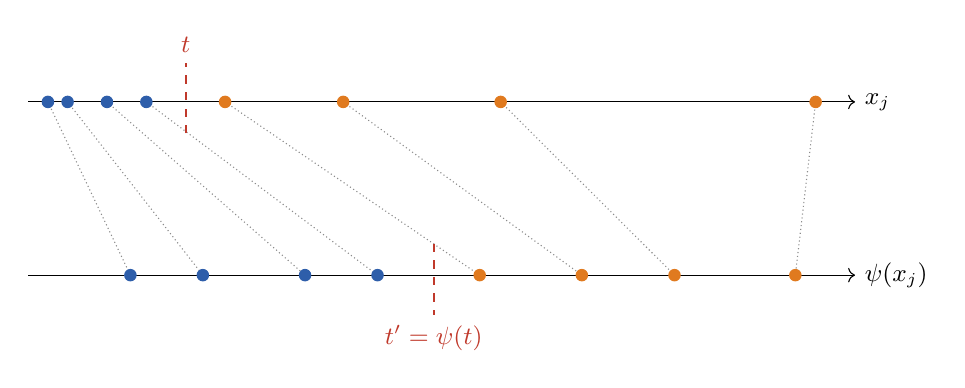
\begin{tikzpicture}[
  izq/.style={circle, fill=azul, inner sep=1.6pt},
  der/.style={circle, fill=naranja, inner sep=1.6pt}]
\draw[->] (0,0) -- (10.5,0) node[right]{\small $x_j$};
\draw[->] (0,-2.2) -- (10.5,-2.2) node[right]{\small $\psi(x_j)$};
\foreach \v in {0.5,1,2,3} {
  \draw[gris, densely dotted] (\v*0.5,0) -- ({ln(\v+1)*3.2},-2.2);
  \node[izq] at (\v*0.5,0) {};
  \node[izq] at ({ln(\v+1)*3.2},-2.2) {};
}
\foreach \v in {5,8,12,20} {
  \draw[gris, densely dotted] (\v*0.5,0) -- ({ln(\v+1)*3.2},-2.2);
  \node[der] at (\v*0.5,0) {};
  \node[der] at ({ln(\v+1)*3.2},-2.2) {};
}
\draw[rojo, thick, dashed] (2,-0.4) -- (2,0.5) node[above]{\small $t$};
\draw[rojo, thick, dashed] ({ln(5)*3.2},-1.8) -- ({ln(5)*3.2},-2.7)
      node[below]{\small $t'=\psi(t)$};
\end{tikzpicture}
\caption{Una transformación creciente (aquí $\log(x+1)$) cambia las distancias
entre puntos pero no su orden. El umbral $t$ y su imagen $t'=\psi(t)$ separan
exactamente los mismos puntos (azul a la izquierda, naranja a la derecha), así
que el árbol encuentra las mismas particiones.}
\label{fig:arbol}
\end{figure}

Por ello, el árbol nos sirve de control, ya que si con la transformación aprendida el error del árbol no cambia, pero el KNN mejora, la mejora viene de la geometría --- las distancias -- que es lo que buscamos demostrar. Si el árbol también cambiara, sospechamos que puede haber fuga de información, preprocesado distinto, etc.

\textsc{Nota}: Si un peso $w_{j}=0$, el atributo se vuelve constante y el árbol ya no puede usarlo. El árbol es invariante siempre que todos los pesos sean mayores que cero. Si en los resultados el árbol empeora un poco, la causa también puede ser que en la búsqueda se ha anulado alguno de los atributos.

\subsection{La transformación aprendida}
Para cada atributo \textit{j} aprendemos dos números: 
\begin{itemize}
    \item Un exponente $\lambda_{j}$, que cambia la forma de la distribución. 
    \item Un peso $w_{j}$ que decide cuánto cuenta ese atributo en la distancia.
\end{itemize}

El proceso por atributo consta de tres pasos visualizados en la \autoref{fig:pipeline}.

\begin{figure}[htbp]
\centering
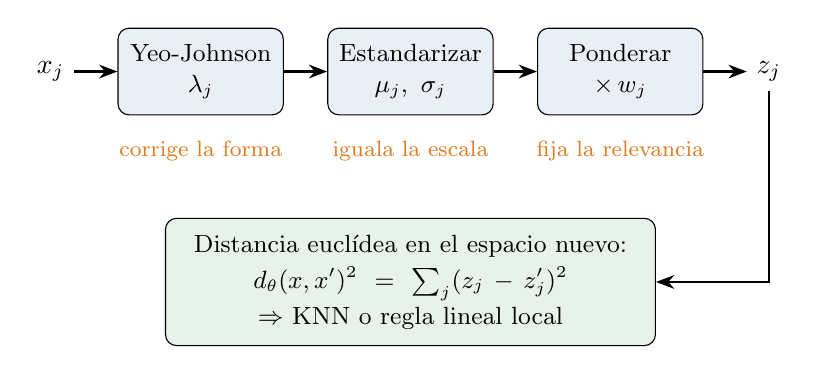
\begin{tikzpicture}[node distance=0.5cm and 0.55cm,
  caja/.style={draw, rounded corners, fill=azul!10, align=center,
               minimum height=1.1cm, minimum width=2.1cm, font=\small},
  flecha/.style={-{Stealth}, thick}]
\node (x) {$x_j$};
\node[caja, right=of x]  (yj) {Yeo-Johnson\\ $\lambda_j$};
\node[caja, right=of yj] (st) {Estandarizar\\ $\mu_j,\ \sigma_j$};
\node[caja, right=of st] (w)  {Ponderar\\ $\times\, w_j$};
\node[right=of w] (z) {$z_j$};
\draw[flecha] (x) -- (yj);
\draw[flecha] (yj) -- (st);
\draw[flecha] (st) -- (w);
\draw[flecha] (w) -- (z);
\node[below=0.2cm of yj, font=\footnotesize, naranja] {corrige la forma};
\node[below=0.2cm of st, font=\footnotesize, naranja] {iguala la escala};
\node[below=0.2cm of w,  font=\footnotesize, naranja] {fija la relevancia};
\node[draw, rounded corners, fill=verde!12, align=center, font=\small,
      text width=5.8cm, inner sep=6pt, below=1.3cm of st] (d)
      {Distancia euclídea en el espacio nuevo:\\[2pt]
       $d_\theta(x,x')^2=\sum_j (z_j-z'_j)^2$\\[2pt]
       $\Rightarrow$ KNN o regla lineal local};
\draw[flecha] (z.south) |- (d.east);
\end{tikzpicture}
\caption{Cada atributo pasa por tres etapas, cada una con un propósito distinto.
Los parámetros aprendidos son $\lambda_j$ y $w_j$; $\mu_j$ y $\sigma_j$ se
calculan con los datos de entrenamiento.}
\label{fig:pipeline}
\end{figure}

\subsubsection{Paso 1: \textit{Yeo-Johnson}}
Yeo-Johnson es una familia de transformaciones de potencia. Según $\lambda$, ''dobla'' el eje del atributo para comprimir o estirar zonas. Es una sucesora de Box-Cox, con una ventaja. En el caso de Yeo-Johnson se aceptan los ceros y negativos. Box-Cox solo funciona con valores positivos, y en California, por ejemplo, tenemos atributos como longitud que son negativos. La fórmula de Yeo-Johnson tiene cuatro casos: 
\begin{enumerate}
    \item Si $x\geq 0\space \text{ y } \lambda \neq 0: \psi=\frac{(x+1)^{\lambda}-1}{\lambda}$
    \item Si $x \geq 0$ y $\lambda =0$: $\psi = \log(x+1)$
    \item Si $x < 0$ y $\lambda \neq 2$: $\psi=-\frac{(-x+1)^{2-\lambda}-1}{2-\lambda}$
    \item Si $x<0$ y $\lambda=2$: $\psi=-\log(-x+1)$
\end{enumerate}

Es importante advertir que los casos con logaritmo no son arbitrarios. Son el límite de la fórmula general cuando $\lambda$ tiende a 0 o a 2. Así la transformación varía de forma suave con $\lambda$, sin saltos, lo cual es bueno para el optimizador. Además, el $+1$ evita problemas con el 0, ya que el $\log(0)$ no existe. Los valores negativos se tratan como un espejo de los positivos, con exponente $2-\lambda$. Para cualquier $\lambda$, la transformación será estrictamente creciente. Nunca cambia el orden. La \autoref{fig:yeojohnson} muestra la curva para varios valores de $\lambda$.

\begin{figure}[htbp]
\centering
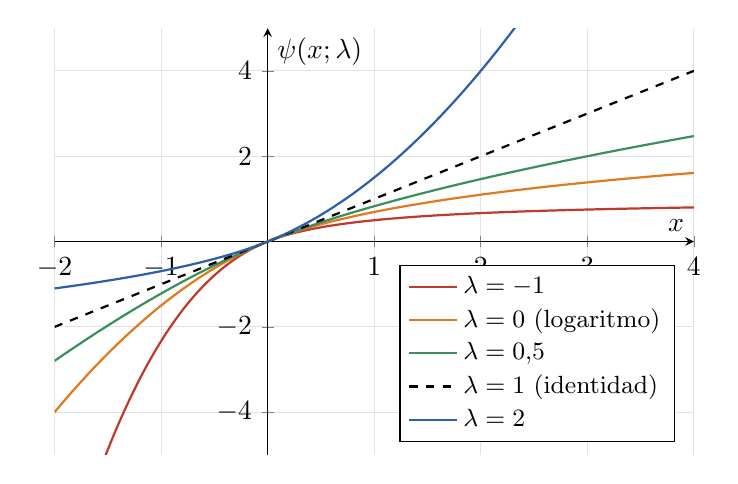
\begin{tikzpicture}
\begin{axis}[width=0.8\textwidth, height=7cm,
  xmin=-2, xmax=4, ymin=-5, ymax=5,
  axis lines=middle, xlabel={$x$}, ylabel={$\psi(x;\lambda)$},
  legend pos=south east, legend cell align=left, legend style={font=\small},
  samples=100, grid=major, grid style={gris!25}]
% lambda = -1
\addplot[rojo, thick, domain=0:4] {1 - 1/(x+1)};
\addlegendentry{$\lambda=-1$}
\addplot[rojo, thick, domain=-2:0, forget plot] {-((1-x)^3 - 1)/3};
% lambda = 0
\addplot[naranja, thick, domain=0:4] {ln(x+1)};
\addlegendentry{$\lambda=0$ (logaritmo)}
\addplot[naranja, thick, domain=-2:0, forget plot] {-((1-x)^2 - 1)/2};
% lambda = 0.5
\addplot[verde, thick, domain=0:4] {2*((x+1)^0.5 - 1)};
\addlegendentry{$\lambda=0{,}5$}
\addplot[verde, thick, domain=-2:0, forget plot] {-((1-x)^1.5 - 1)/1.5};
% lambda = 1
\addplot[black, thick, dashed, domain=-2:4] {x};
\addlegendentry{$\lambda=1$ (identidad)}
% lambda = 2
\addplot[azul, thick, domain=0:4] {((x+1)^2 - 1)/2};
\addlegendentry{$\lambda=2$}
\addplot[azul, thick, domain=-2:0, forget plot] {-ln(1-x)};
\end{axis}
\end{tikzpicture}
\caption{Transformación de Yeo-Johnson para varios $\lambda$. Con $\lambda=1$ es
la identidad (línea discontinua). Con $\lambda<1$ la curva se aplana para $x$
grandes: comprime la cola derecha. Con $\lambda>1$ se empina: la estira. Todas las
curvas son crecientes, así que nunca cambian el orden de los datos.}
\label{fig:yeojohnson}
\end{figure}

\textsc{¿Qué hace cada valor de $\lambda$?}

\begin{itemize}
    \item $\lambda=1$: es la identidad, no cambia nada. Sirve cuando los atributos están ya bien distribuidos. 
    \item $\lambda < 1$: comprime los valores grandes, lo cual es útil cuando tenemos colas  largas a la derecha. 
    \item $\lambda = 0$: logaritmo para valores mayores o iguales que cero. Esto sirve además en presencia de datos muy sesgados.
    \item $\lambda>1$: estira los valores grandes, útil en presencia de colas a la izquierda.
\end{itemize}

\textsc{Importante}: Yeo-Johnson suele usarse para datos que sigan o se parezcan a una normal. Se estima $\lambda$ por máxima verosimilitud. Nosotros lo que hacemos, por el contrario es elegir $\lambda$ de manera que la distancia prediga bien, que es un objetivo distinto. Por eso el valor de $\lambda$ lo busca CMA-ES.

\subsubsection{Paso 2 y 3: estandarizar y ponderar}
Después de transformar, centramos y escalamos con la media $\mu_{j}$ y la desviación estándar $\sigma_{j}$ calculadas en el entrenamiento, y multiplicamos por el peso. 

$$ 
z_{j} = w_{j} \cdot \frac{\psi(x_{j}; \lambda_{j})-\mu_{j}}{\sigma_{j}}
$$

Estandarizar lo que hace es poner todos los atributos en la misma escala, por lo que el peso pasa a ser lo único que decida la importancia. Se usan $\mu$ y $\sigma$ del entrenamiento para no filtrar los datos del test. 

\textsc{¿Qué significa esto para la distancia?}

Si llamamos $\tilde{x_{j}}$ al atributo transformado y estandarizado --- antes del peso --- la distancia euclídea en el nuevo espacio se define como: 

$$ 
d_{\theta}(x, x')^2=\sum_{j}w_{j}^2 \cdot (\tilde{x_{j}}-\tilde{x_{j}'})^2
$$

Pasa a ser una distancia ponderada, donde cada atributo contribuye con la importancia $w_{j}^2$. Si el peso se reduce el cero, el atributo desaparece. Es una selección de atributos automática: el optimizador puede apagar los irrelevantes. Y si el peso es muy grande, ese atributo dominará en las distancias. 

Si repartiéramos las tareas: 
\begin{itemize}
    \item El $\lambda$ arregla la forma --- problema 3. 
    \item Estandarizar arregla la escala --- problema 1. 
    \item Los pesos arreglan la relevancia --- problema 2.
\end{itemize}

\subsubsection{Conexión con la teoría de métricas}
Una distancia de Mahalanobis general es de: 
$$ 
d^2  = (x-x')^{T} M (x-x')
$$

Donde $M$ es una matriz que puede mezclar atributos. Nuestra M es diagonal, con valores que van desde $w_{1}^2 \cdots w_{n}^2$. En este caso no estamos mezclando atributos, pero sí que los estamos ponderando. Además, se aplica después de una transformación no lineal por atributo. Por eso podemos decir que aprendemos una métrica diagonal con transformación previa. Es menos expresiva que una M completa (\autoref{fig:mahalanobis}), pero tiene muchos menos parámetros ($2n$ en lugar de unos $\frac{n^2}{2}$). Esto reduce el sobreajuste y la hace interpretable, ya que puedes leer qué atributo importa mirando su peso. 

\begin{figure}[htbp]
\centering
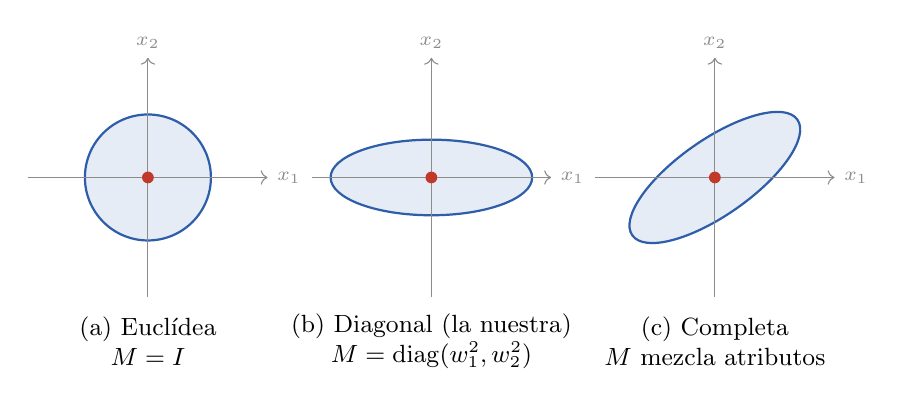
\begin{tikzpicture}[scale=0.8]
\foreach \dx/\titulo/\rx/\ry/\rot in {
   0/{(a) Euclídea\\ $M=I$}/1/1/0,
   4.5/{(b) Diagonal (la nuestra)\\ $M=\mathrm{diag}(w_1^2,w_2^2)$}/1.6/0.6/0,
   9/{(c) Completa\\ $M$ mezcla atributos}/1.6/0.6/35}{
  \begin{scope}[xshift=\dx cm]
    \draw[azul, thick, fill=azul!12, rotate=\rot] (0,0) ellipse ({\rx} and {\ry});
    \draw[->, gris] (-1.9,0) -- (1.9,0) node[right]{\scriptsize $x_1$};
    \draw[->, gris] (0,-1.9) -- (0,1.9) node[above]{\scriptsize $x_2$};
    \node[circle, fill=rojo, inner sep=1.5pt] at (0,0) {};
    \node[align=center, font=\small] at (0,-2.6) {\titulo};
  \end{scope}
}
\end{tikzpicture}
\caption{Puntos a distancia 1 del centro según el tipo de métrica. La euclídea
trata todas las direcciones igual. La diagonal estira o encoge cada eje por
separado, pero los ejes de la elipse siguen alineados con los atributos. La
completa puede además rotar la elipse, combinando atributos, a costa de muchos
más parámetros.}
\label{fig:mahalanobis}
\end{figure}

\subsubsection{El vector de parámetros}
Lo que buscamos al final es un $\theta = (\lambda_{1}\cdots \lambda_{n}, w_{1}, \cdots w_{n})$. Siendo el punto de partida $\theta=(1...1)$. Es decir, con todos los $\lambda=1$ (identidad) y todos los $w=1$(sin ponderación), o lo que es estandarización normal. La búsqueda no empieza en un punto aleatorio, que sí que podría llegar a ser peor que la estandarización. 

\textsc{Limitación de $\lambda$}: limitamos los valores de $\lambda$ porque sin límites, el estimador de máxima verosimilitud de Yeo-Johnson dio un $\lambda\approx 13,6$ para el atributo de longitud de California. Esto falla porque: 
\begin{itemize}
    \item La longitud de California no tiene una forma simple, si vemos su histograma, es una variable bimodal. El estimador lo que hace es forzar una normal, yendo a valores extremos. 
    \item Además, como las coordenadas pueden ser negativas, se usa la rama del exponente de $2-\lambda=-11,6$. Elevar a números del orden de 120 a -11,6 da valores prácticamente cero para todos, por lo que toda columna colapsa cerca de un único valor (-0,0862) con diferencias del orden de $10^{25}$. Esto lo podemos ver en la \autoref{fig:colapso}.
\end{itemize}

\begin{figure}[htbp]
\centering
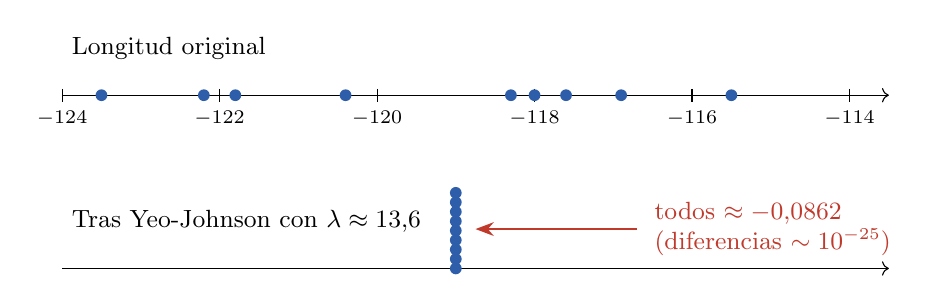
\begin{tikzpicture}[pt/.style={circle, fill=azul, inner sep=1.5pt}]
% Original
\node[anchor=west, font=\small] at (0,0.6) {Longitud original};
\draw[->] (0,0) -- (10.5,0);
\foreach \v in {-124,-122,-120,-118,-116,-114} {
  \draw ({\v+124},0.08) -- ({\v+124},-0.08) node[below]{\scriptsize $\v$};
}
\foreach \v in {-123.5,-122.2,-121.8,-120.4,-118.3,-118,-117.6,-116.9,-115.5} {
  \node[pt] at ({\v+124},0) {};
}
% Transformada
\begin{scope}[yshift=-2.2cm]
\node[anchor=west, font=\small] at (0,0.6) {Tras Yeo-Johnson con $\lambda \approx 13{,}6$};
\draw[->] (0,0) -- (10.5,0);
\foreach \k in {0,...,8} { \node[pt] at (5,0.12*\k) {}; }
\draw[rojo, thick, -{Stealth}] (7.3,0.5) -- (5.25,0.5);
\node[anchor=west, font=\small, rojo, align=left] at (7.4,0.5)
     {todos $\approx -0{,}0862$\\ (diferencias $\sim 10^{-25}$)};
\end{scope}
\end{tikzpicture}
\caption{Con $\lambda \approx 13{,}6$, los valores negativos de la longitud se
elevan a $2-\lambda=-11{,}6$, lo que da números prácticamente nulos. Todos los
puntos acaban en el mismo valor y el atributo deja de servir para medir
distancias. Limitar $\lambda\in[-2,2]$ lo evita.}
\label{fig:colapso}
\end{figure}

Con $\lambda\in[-2,2]$ la transformación puede comprimir o estirar con fuerza, pero nunca hasta destruir el atributo.

\subsection{CMA-ES: cómo buscamos $\theta$}
\subsubsection{Qué problema resolvemos}

Tenemos una función $f(\theta)$ que nos dice lo bueno que es cada $\theta$ (el fitness), y queremos que $\theta$ la minimice. Pero: 
\begin{itemize}
    \item No tiene gradiente: depende de qué puntos acaban siendo vecinos de los otros. Y esto cambia a saltos. 
    \item Cada evaluación es cara, porque hay que hacer validazión cruzada entera. 
    \item Tiene algo de ruido, por lo que pueden haber varios mínimos locales.
\end{itemize}

CMA-ES (Covariance Matrix Adaptation Evolution Strategy, Hansen y Ostermeier, 2001) es una estrategia evolutiva pensada para esto. Optimización continua, sin gradiente, en dimensiones moderadas (de unas pocas a cientos de variables). 

\subsubsection{La idea intuitiva}
En vez de mantener una población de soluciones sueltas, CMA-ES mantiene una distribución normal multivariante que representa ''dónde creo que está el óptimo''. Tenemos tres elementos: 
\begin{enumerate}
    \item $m$(media): el centro, la mejor estimación actual. 
    \item $\sigma$(el tamaño de paso): cuánto se aleja al explorar. Es la escala global. 
    \item $C$(matriz de covarianza): la forma de la nube de búsqueda. Puede ser alargada, inclinada, etc; explorando más en unas direcciones que en otras.
\end{enumerate}

Es una nube de exploración que se mueve hacia las zonas buenas, se encoge cuando se encuentra cerca del óptimo y se deforma para alinearse con aquellas direcciones más prometedoras. 

\textsc{Aclaración} En el caso del CMA-ES, el $\lambda$ es el tamaño de la población, no tiene nada que  ver con los $\lambda$ de Yeo-Johnson. Por eso la vamos a denominar $\lambda_{pop}$. 

\subsubsection{Una generación, paso a paso.}

Una generación de CMA-ES agrupa los siguientes pasos, visualizados en la \autoref{fig:cmaciclo}.

\begin{figure}[htbp]
\centering
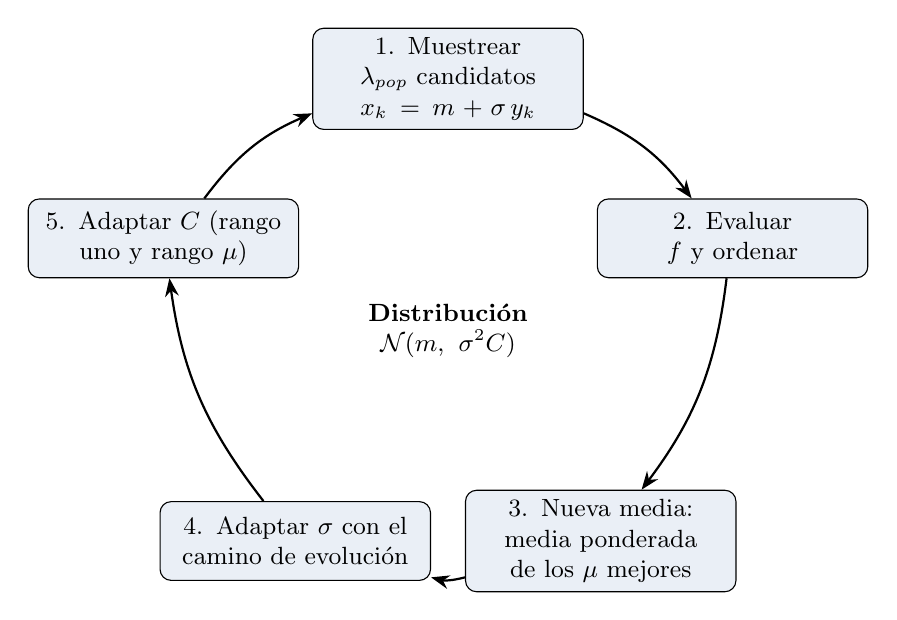
\begin{tikzpicture}[
  paso/.style={draw, rounded corners, fill=azul!10, align=center,
               text width=3.2cm, font=\small, minimum height=1cm},
  flecha/.style={-{Stealth}, thick}]
\node[paso] (a) at (90:3.2)   {1. Muestrear $\lambda_{pop}$ candidatos\\ $x_k = m + \sigma\, y_k$};
\node[paso] (b) at (18:3.8)   {2. Evaluar $f$ y ordenar};
\node[paso] (c) at (-54:3.3)  {3. Nueva media: media ponderada de los $\mu$ mejores};
\node[paso] (d) at (-126:3.3) {4. Adaptar $\sigma$ con el camino de evolución};
\node[paso] (e) at (162:3.8)  {5. Adaptar $C$ (rango uno y rango $\mu$)};
\node[align=center, font=\small\bfseries] at (0,0) {Distribución\\ $\mathcal{N}(m,\ \sigma^2 C)$};
\draw[flecha] (a) to[bend left=15] (b);
\draw[flecha] (b) to[bend left=15] (c);
\draw[flecha] (c) to[bend left=15] (d);
\draw[flecha] (d) to[bend left=15] (e);
\draw[flecha] (e) to[bend left=15] (a);
\end{tikzpicture}
\caption{Una generación de CMA-ES. Toda la información se guarda en la
distribución normal $\mathcal{N}(m,\sigma^2 C)$: los pasos 3, 4 y 5 actualizan
su centro, su tamaño y su forma.}
\label{fig:cmaciclo}
\end{figure}

\begin{enumerate}
    \item \textbf{Muestrear}. Se generan $\lambda_{pop}$ candidatos alrededor de la media $x_{k}=m+\sigma\cdot y_{k}$, con $y_{k}\sim N(0,C)$.
    \item \textbf{Evaluar y ordenar}: Se calcula el fitness de cada uno y se ordena de mejor a peor. 
    \item \textbf{Seleccionar y recombinar}: Se quedan con los $\mu$ mejores (por defecto la mitad) y la nueva media es una \textbf{media ponderada} de ellos, con más peso al mejor. La nube se desplaza hacia donde están los buenos. 
    \item \textbf{Adaptar $\sigma$}: CMA-ES guarda un camino de evolución, es decir, la suma acumulada de los últimos desplazamientos de la media. Esto se representa en la \autoref{fig:camino}. Si todos los pasos van en la misma dirección, el camino es largo, por lo que vamos lento y conviene aumentar la $\sigma$. Sin embargo, si los caminos se cancelan, el camino es corto. Estamos dando vueltas alrededor del óptimo, por lo que nos conviene reducir el valor de $\sigma$. 
    
    \begin{figure}[htbp]
    \centering
    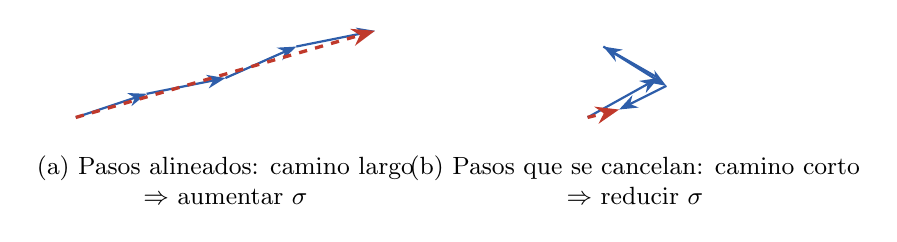
\begin{tikzpicture}[paso/.style={-{Stealth}, thick, azul},
                        total/.style={-{Stealth}, very thick, rojo, dashed}]
    % (a) Pasos alineados
    \draw[paso] (0,0) -- (0.9,0.3);
    \draw[paso] (0.9,0.3) -- (1.9,0.5);
    \draw[paso] (1.9,0.5) -- (2.8,0.9);
    \draw[paso] (2.8,0.9) -- (3.8,1.1);
    \draw[total] (0,0) -- (3.8,1.1);
    \node[align=center, font=\small] at (1.9,-0.8)
        {(a) Pasos alineados: camino largo\\ $\Rightarrow$ aumentar $\sigma$};
    % (b) Pasos que se cancelan
    \begin{scope}[xshift=6.5cm]
    \draw[paso] (0,0) -- (0.9,0.5);
    \draw[paso] (0.9,0.5) -- (0.2,0.9);
    \draw[paso] (0.2,0.9) -- (1.0,0.4);
    \draw[paso] (1.0,0.4) -- (0.4,0.1);
    \draw[total] (0,0) -- (0.4,0.1);
    \node[align=center, font=\small] at (0.6,-0.8)
        {(b) Pasos que se cancelan: camino corto\\ $\Rightarrow$ reducir $\sigma$};
    \end{scope}
    \end{tikzpicture}
    \caption{Pasos sucesivos de la media (azul) y su suma acumulada, el camino de
    evolución (rojo). Si el camino es más largo de lo esperado por azar, el paso es
    demasiado pequeño; si es más corto, demasiado grande.}
    \label{fig:camino}
    \end{figure}

    \item \textbf{Adaptamos el C} con dos actualizaciones: 
    \begin{enumerate}
        \item Rango uno - usa el camino de evolución para estirar la nube en la dirección por la que se viene avanzando de forma consistente. 
        \item Rango $\mu$: usa los $\mu$ mejores de la generación para aprender la forma de la región nueva.
    \end{enumerate}
\end{enumerate}

\subsubsection{Qué ganamos con C}

Si dos parámetros están correlacionados --- por ejemplo, subir el peso de un atributo solo funciona si a la vez cambias su $\lambda$ --- C lo aprende y propone cambios conjuntos. Si un parámetro necesita pasos mucho más pequeños que otro, C también lo aprende. Es como aprender un ''reescalado'' del problema, y por eso CMA-ES funciona bien en problemas mal condicionados (\autoref{fig:cmaelipses}).

\begin{figure}[htbp]
\centering
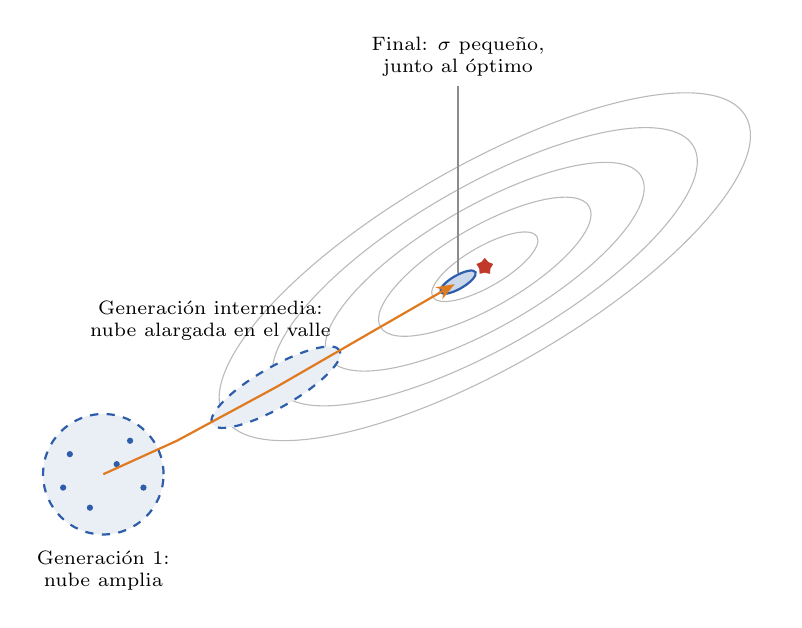
\begin{tikzpicture}[scale=0.85]
% Curvas de nivel de la función (valle inclinado)
\begin{scope}[shift={(7,3.5)}, rotate=30]
  \foreach \k in {1,...,5} { \draw[gris!60] (0,0) ellipse ({0.9*\k} and {0.3*\k}); }
  \node[star, star points=5, fill=rojo, inner sep=1.5pt] at (0,0) {};
\end{scope}
% Generación 1: nube amplia y redonda
\draw[azul, thick, dashed, fill=azul!10] (1.3,0.4) circle (0.9);
\foreach \p in {(0.8,0.7),(1.7,0.9),(1.1,-0.1),(1.9,0.2),(0.7,0.2),(1.5,0.55)} {
  \node[circle, fill=azul, inner sep=0.8pt] at \p {};
}
% Generación intermedia: alargada en la dirección del valle
\draw[azul, thick, dashed, fill=azul!10, rotate around={30:(3.88,1.7)}]
     (3.88,1.7) ellipse (1.1 and 0.3);
% Final: pequeña junto al óptimo
\draw[azul, thick, fill=azul!25, rotate around={30:(6.6,3.27)}]
     (6.6,3.27) ellipse (0.3 and 0.1);
% Trayectoria de la media
\draw[-{Stealth}, thick, naranja] (1.3,0.4) -- (2.4,0.9) -- (3.88,1.7)
      -- (5.3,2.52) -- (6.55,3.24);
% Etiquetas
\node[font=\scriptsize, align=center, below] at (1.3,-0.6) {Generación 1:\\ nube amplia};
\node[font=\scriptsize, align=center] at (2.9,2.7) {Generación intermedia:\\ nube alargada en el valle};
\node[font=\scriptsize, align=center, above] at (6.6,6.2) {Final: $\sigma$ pequeño,\\ junto al óptimo};
\draw[gris] (6.6,6.2) -- (6.6,3.4);
\end{tikzpicture}
\caption{Esquema de la búsqueda sobre una función con un valle inclinado (curvas
de nivel en gris, óptimo en rojo). La nube empieza amplia, se alarga en la
dirección del valle gracias a $C$ y se encoge al acercarse al óptimo gracias a
$\sigma$. La línea naranja es la trayectoria de la media $m$.}
\label{fig:cmaelipses}
\end{figure}

\subsubsection{Por qué nos conviene CMA-ES}

En primer lugar, porque no necesita gradiente. Nuestro fitness incluye  búsqueda de vecinos y ajustes locales, que no son derivables. Además, usa el orden de los candidatos, no el valor del fitness. Si un fitness pasara de 0,4 a 0,41 o a 100, si el orden es el mismo, CMA-ES opera de la misma manera. Es invariante a transformaciones monótonas del fitness y bastante robusto al ruido (pequeñas variaciones solo importan si cambian el orden). Finalmente, casi no hace falta ajustarlo. Aprende la forma del problema él solo. El tamaño de población por defecto es $\lambda_{pop}=4+\rfloor 3 \cdot \ln D\lfloor$. En el caso de California son 12 candidatos por generación, y en diabetes también. Con 1.000 evaluaciones tendremos un total de 83 generaciones. 

\subsubsection{Implementación}
En la práctica usamos una implementación propia. En la extensión usamos la librería de referencia \texttt{cma} (de Hansen), donde obtenemos resultados equivalentes, lo que nos permite también validar nuestra implementación. 

Trabajamos en el cubo normalizado de $[0,1]^D$. Cada parámetro se mapea a [0,1] y se reescala a sus límites reales al evaluar. Así todos los parámetros tienen la misma escala inicial y un único $\sigma$ inicial tiene sentido para todos. El punto de partida $\theta_{0}$ se corresponde a 0,75 para cada $\lambda$ (1 está a 3/4 del camino entre -2 y 2) y a 1/3 para cada w. 

\subsection{El fitness: cómo sabe la búsqueda si un $\theta$ es bueno}
\subsubsection{Procedimiento}

\begin{figure}[htbp]
\centering
% (a) Flujo
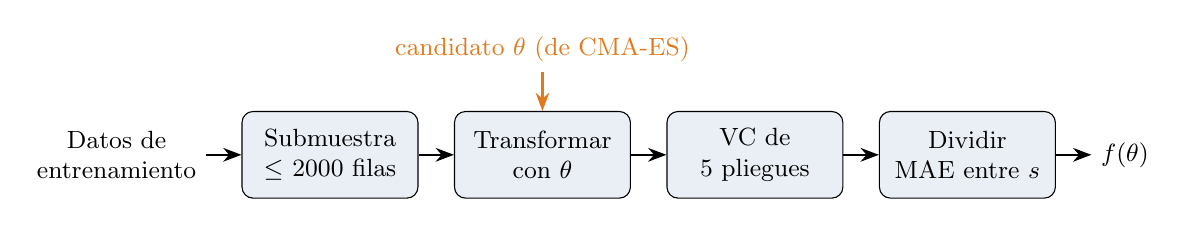
\begin{tikzpicture}[node distance=0.45cm,
  caja/.style={draw, rounded corners, fill=azul!10, align=center,
               text width=2cm, minimum height=1.1cm, font=\small},
  flecha/.style={-{Stealth}, thick}]
\node[font=\small, align=center] (ent) {Datos de\\ entrenamiento};
\node[caja, right=of ent] (sub) {Submuestra\\ $\le 2000$ filas};
\node[caja, right=of sub] (tr)  {Transformar\\ con $\theta$};
\node[caja, right=of tr]  (vc)  {VC de\\ 5 pliegues};
\node[caja, right=of vc]  (nor) {Dividir\\ MAE entre $s$};
\node[right=of nor, font=\small] (f) {$f(\theta)$};
\draw[flecha] (ent) -- (sub);
\draw[flecha] (sub) -- (tr);
\draw[flecha] (tr) -- (vc);
\draw[flecha] (vc) -- (nor);
\draw[flecha] (nor) -- (f);
\node[above=0.5cm of tr, font=\small, naranja] (th) {candidato $\theta$ (de CMA-ES)};
\draw[flecha, naranja] (th) -- (tr);
\end{tikzpicture}

\bigskip

% (b) Pliegues
\begin{tikzpicture}[x=1.1cm, y=0.55cm]
\foreach \i in {1,...,5} {
  \foreach \j in {1,...,5} {
    \ifnum\i=\j \def\colorpliegue{naranja!70}\else \def\colorpliegue{azul!20}\fi
    \fill[fill=\colorpliegue, draw=white, thick] (\j-1,-\i) rectangle (\j,-\i+0.85);
  }
  \node[anchor=east, font=\small] at (-0.1,-\i+0.42) {Pliegue \i};
  \node[anchor=west, font=\small] at (5.1,-\i+0.42) {$\mathrm{MAE}_{\i}$};
}
\fill[azul!20] (0,-6.4) rectangle (0.4,-6.0);
\node[anchor=west, font=\small] at (0.45,-6.2) {entrenar};
\fill[naranja!70] (2.4,-6.4) rectangle (2.8,-6.0);
\node[anchor=west, font=\small] at (2.85,-6.2) {evaluar};
\node[font=\small] at (2.5,-7.4)
     {$f(\theta)=\dfrac{1}{5}\displaystyle\sum_{i=1}^{5}\dfrac{\mathrm{MAE}_i}{s}$};
\end{tikzpicture}
\caption{(a) Flujo para evaluar un candidato $\theta$. (b) Validación cruzada
de 5 pliegues: en cada fila se entrena con cuatro bloques (azul) y se mide el
error en el restante (naranja). El fitness es la media de los cinco errores,
normalizados por el error del predictor trivial.}
\label{fig:fitness}
\end{figure}

El procedimiento se resume en la \autoref{fig:fitness}. Para cada candidato $\theta$: 
\begin{enumerate}
    \item Subustreo: se toman gasta 2000 filas del entrenamiento para que cada evaluación sea rápida. 
    \item Transformación: se aplica $\theta$ con $\mu$ y $\sigma$ calculadas sobre esas filas. 
    \item Validación cruzada de cinco pliegues: se divide en 5 partes; 5 veces se entrenan con 4, y se mide el MAE (error absoluto medio) en la restante. 
    \item Normalización: cada MAE se divide entre $s$, el error de un predictor trivial que siempre predice la mediana.
\end{enumerate}

\subsubsection{Cómo leemos el fitness}
Es el error como fracción del error de no saber nada (\autoref{fig:escalafitness})

\begin{itemize}
    \item $f=1$: el modelo es tan malo como predecir siempre la mediana. 
    \item $f=0,5$: comete la mitad de error que un predictor sin información. 
    \item $f=0$: perfecto
\end{itemize}

\begin{figure}[htbp]
\centering
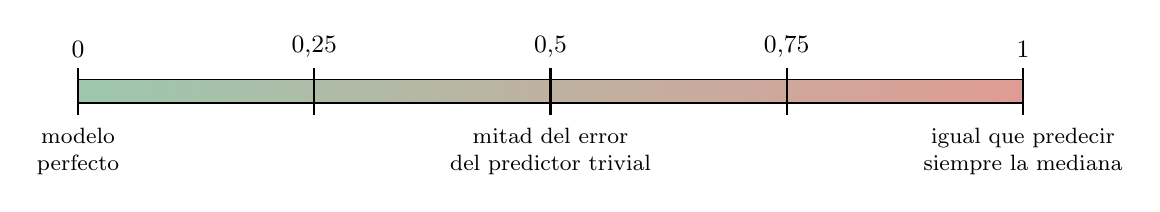
\begin{tikzpicture}
\shade[left color=verde!50, right color=rojo!50] (0,-0.15) rectangle (12,0.15);
\draw (0,-0.15) rectangle (12,0.15);
\draw[thick] (0,0.3) -- (0,-0.3);
\draw[thick] (3,0.3) -- (3,-0.3);
\draw[thick] (6,0.3) -- (6,-0.3);
\draw[thick] (9,0.3) -- (9,-0.3);
\draw[thick] (12,0.3) -- (12,-0.3);
\node[above, font=\small] at (0,0.3)  {$0$};
\node[above, font=\small] at (3,0.3)  {$0{,}25$};
\node[above, font=\small] at (6,0.3)  {$0{,}5$};
\node[above, font=\small] at (9,0.3)  {$0{,}75$};
\node[above, font=\small] at (12,0.3) {$1$};
\node[below, font=\footnotesize, align=center] at (0,-0.35)  {modelo\\ perfecto};
\node[below, font=\footnotesize, align=center] at (6,-0.35)  {mitad del error\\ del predictor trivial};
\node[below, font=\footnotesize, align=center] at (12,-0.35) {igual que predecir\\ siempre la mediana};
\end{tikzpicture}
\caption{Escala del fitness $f(\theta)$. Al expresarse como fracción del error
del predictor trivial, es comparable entre datasets con escalas distintas.}
\label{fig:escalafitness}
\end{figure}


\textsc{Por qué usamos la mediana}: es la constante que minimiza el error absoluto, así que es la referencia natural para el MAE (para el error cuadrático sería la media). 

\textsc{Por qué normalizar}: Un MAE de 0,4 en precios de vivienda que se mide en miles de dólares, no es comparable con un MAE de 40 en Diabetes. Al dividir entre $s$, ambos se expresan en la misma escala relativa y podemos comparar datasets. 

\textsc{Qué modelo usa}: en el notebook principal, el fitness promedia regresión lineal y KNN. En la extensión usa el modelo para el que optimizamos: KNN o la regla local lineal. 

\subsubsection{El riesgo: sobreajustar el fitness}
La búsqueda lo que hace es optimizar una estimación del error, no el error real. Con 1000 evaluaciones, probando muchos $\theta$ distintos, acaba encontrando alguno que funciona especialmente bien en esos pliegues en concreto, en parte por casualidad. Es la maldición del ganador, si elegimos el mejor de muchos candidatos ruidosos, su puntuación está inflada. Cuando hay pocos datos, cada pliegue tiene unas 60 filas y el ruido es gande. La búsqueda aprende ese ruido: el fitness mejora en entrenamiento, pero no en la validación. Esto lo vemos en la \autoref{fig:sobreajuste}. Este es el problema principal de Diabetes, y es una conclusión valiosa. El método necesita suficientes datos para que el fitness sea fiable. Formas de mitigarlo podrían ser: repetir la validación cruzada con varias particiones, regularizar $\theta$ hacia $\theta_{0}$ o reducir el número de parámetros (por ejemplo, solo pesos).

\begin{figure}[htbp]
\centering
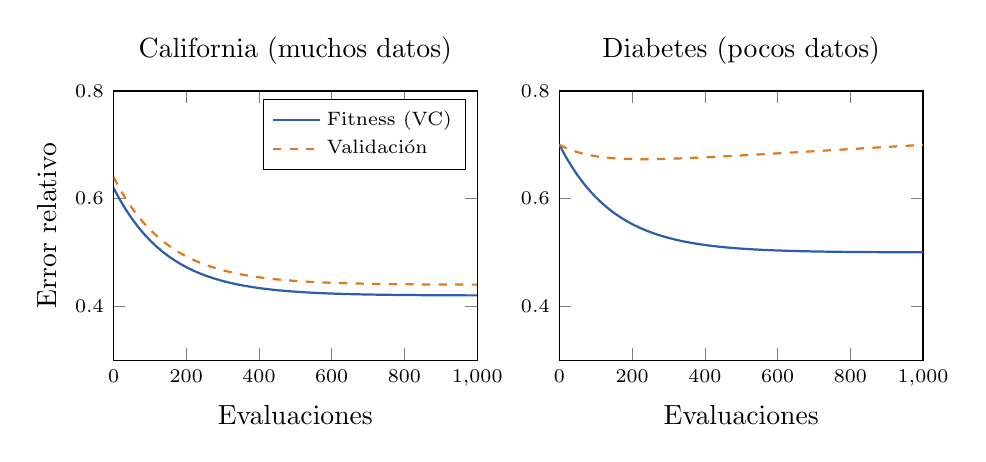
\begin{tikzpicture}
\begin{axis}[name=cal, width=6.2cm, height=5cm,
  title={California (muchos datos)}, xlabel={Evaluaciones}, ylabel={Error relativo},
  xmin=0, xmax=1000, ymin=0.3, ymax=0.8, domain=0:1000, samples=60,
  ticklabel style={font=\scriptsize}, legend style={font=\scriptsize},
  legend pos=north east, legend cell align=left]
\addplot[azul, thick] {0.42 + 0.2*exp(-x/150)};
\addlegendentry{Fitness (VC)}
\addplot[naranja, thick, dashed] {0.44 + 0.2*exp(-x/150)};
\addlegendentry{Validación}
\end{axis}
\begin{axis}[at={(cal.outer east)}, anchor=outer west, width=6.2cm, height=5cm,
  title={Diabetes (pocos datos)}, xlabel={Evaluaciones},
  xmin=0, xmax=1000, ymin=0.3, ymax=0.8, domain=0:1000, samples=60,
  ticklabel style={font=\scriptsize}]
\addplot[azul, thick] {0.5 + 0.2*exp(-x/150)};
\addplot[naranja, thick, dashed] {0.66 + 0.04*exp(-x/100) + 0.00004*x};
\end{axis}
\end{tikzpicture}
\caption{Esquema ilustrativo (no son datos reales). Con muchos datos, el fitness
y el error de validación bajan juntos. Con pocos datos, la búsqueda sigue
bajando el fitness, pero la validación no mejora: está aprendiendo el ruido de
los pliegues.}
\label{fig:sobreajuste}
\end{figure}

\subsection{La regla de predicción: de KNN a regresión lineal local}
\subsubsection{El límite de KNN}
KNN predice con la media de los vecinos, es decir, supone que la función es plana en el entorno de $q$. Por eso se le llama regresión local constante. El problema es que si la función tiene pendiente en esa zona, la media de los vecinos se desvía. Y es peor en los bordes de los datos: si $q$ está en el extremo --- por ejemplo, en el barrio con renta más alta --- todos sus vecinos tienen renta más baja, todos tienen precio más bajo y KNN subestima sistemáticamente. Esto se le llama \textbf{sesgo de borde} y lo podemos visualizar en \autoref{fig:sesgoborde}.

\begin{figure}[htbp]
\centering
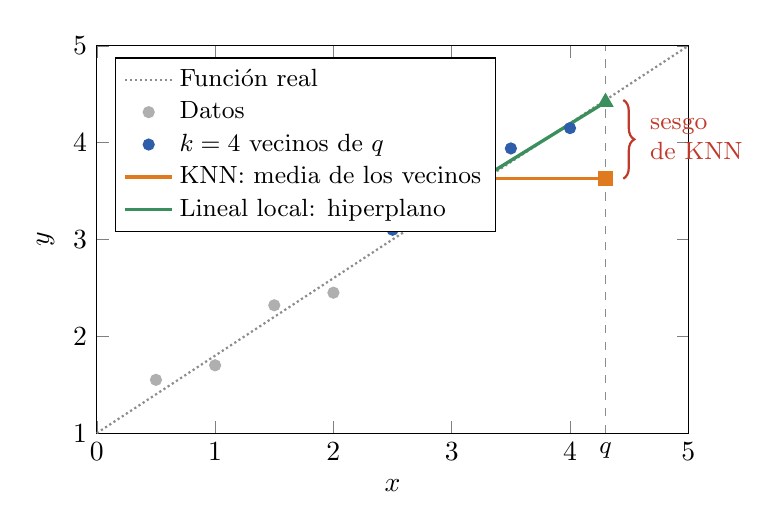
\begin{tikzpicture}
\begin{axis}[width=0.75\textwidth, height=6.5cm, clip=false,
  xmin=0, xmax=5, ymin=1, ymax=5, xlabel={$x$}, ylabel={$y$},
  legend pos=north west, legend cell align=left, legend style={font=\small}]
\addplot[gris, densely dotted, thick, domain=0:5] {1 + 0.8*x};
\addlegendentry{Función real}
\addplot[only marks, mark=*, gris!70]
  coordinates {(0.5,1.55) (1,1.70) (1.5,2.32) (2,2.45)};
\addlegendentry{Datos}
\addplot[only marks, mark=*, azul]
  coordinates {(2.5,3.10) (3,3.32) (3.5,3.94) (4,4.15)};
\addlegendentry{$k=4$ vecinos de $q$}
\addplot[naranja, very thick, domain=2.5:4.3] {3.6275};
\addlegendentry{KNN: media de los vecinos}
\addplot[verde, very thick, domain=2.5:4.3] {3.6275 + 0.754*(x-3.25)};
\addlegendentry{Lineal local: hiperplano}
\draw[dashed, gris] (axis cs:4.3,1) -- (axis cs:4.3,5);
\node[below, font=\small] at (axis cs:4.3,1) {$q$};
\addplot[only marks, mark=square*, naranja, mark size=2.5pt, forget plot]
  coordinates {(4.3,3.6275)};
\addplot[only marks, mark=triangle*, verde, mark size=3pt, forget plot]
  coordinates {(4.3,4.419)};
\draw[decorate, decoration={brace, amplitude=4pt}, rojo, thick]
  (axis cs:4.45,4.44) -- (axis cs:4.45,3.6275)
  node[midway, right=6pt, font=\small, align=left] {sesgo\\ de KNN};
\end{axis}
\end{tikzpicture}
\caption{El punto $q$ está en el borde de los datos y todos sus vecinos quedan a
su izquierda. KNN predice su media (cuadrado naranja), que subestima el valor
real. La regresión lineal local ajusta una recta a los mismos vecinos y la
evalúa en $q$ (triángulo verde), con lo que recupera la tendencia y casi
elimina el sesgo.}
\label{fig:sesgoborde}
\end{figure}

\subsubsection{La regresión lineal local}
La idea es que en vez de suponer la función plana alrededor de $q$, la suponemos lineal. Por ende, para cada $q$: 
\begin{enumerate}
    \item Se buscan sus \textit{k} vecinos $z_{j}$ con valores $y_{j}$. 
    \item Se ajusta un hiperplano solo con esos vecinos. 
    \item Se evalúa un hiperplano en \textit{q}. 
\end{enumerate}

En la \autoref{fig:sesgoborde} podemos ver el sesgo del borde. El ajuste lo que minimiza: 
$$ 
\sum_{i}w_{i} \cdot (y_{i}-\beta_{0}+\beta^T(z_{i}-q))^2 + r \cdot \overline{x} \cdot || \beta ||^2 
$$

Por partes: 
\begin{itemize}
    \item $\beta_{0}+\beta^T(z_{i}-q)$ es el hiperplano. Donde $\beta_{0}$ es la altura y $\beta$ la pendiente en cada dirección. 
    \item $(z_{i}-q)$: se centra en \textit{q}. Así, al evaluar en \textit{q}, el término dependiente se anula y la predicción es directamente $\beta_{0}$. 
    \item $w_{i}$ es el peso de cada vecino --- los cercanos cuentan más. 
    \item $r\cdot \overline{w}\cdot ||\beta||^2$ es la penalización ridge sobre la pendiente.
\end{itemize}

Es un problema de mínimos cuadrados ponderados con solución cerrada : un sistema lineal pequeño por consulta. Esto reduce el sesgo porque si la función es aproximadamente lineal cerca de \textit{q}, el hiperplano captura esa pendiente y el sesgo de borde desaparece. En la teoría de regresión no paramétrica se demuestra que la regresión local lineal tiene el mismo orden de sesgo en el borde que en el interior. Mientras que la local constante (KNN) tiene un sesgo mayor en los bordes. 

\subsubsection{Los tres componentes}
\textsc{Pesos tricúbicos}

$$ 
w_{i} = (1-u_{i}^3)^3 \text{ con } u_{i} = \frac{d_{i}}{d_{max}}
$$

Donde $d_{i}$ es la distancia del vecino \textit{i} 
\newpage
\section{Código del método}
\begin{enumerate}
    \item Primero se realiza la configuración y se establece el estilo de las gráficas.
    \item Carga de los datos, se descargan también 10 datasets de OpenML. Nos quedamos solo con atributos numéricos y si un dataset tiene más de 10.000 filas, usamos submuestra fija de 10.000 para que el coste sea comparable.
    \item \texttt{ajustar(xt, theta) }recibe el entrenamiento y un vector $\theta=(\lambda, w)$ y devuelve una función `v` que transforma cualquier conjunto de datos. Lo importante es que la media y la desviación se calculan solo con el entrenamiento y se reutilizan para la validación.
    \item Para las reglas de predicción tenemos KNN y regresión lineal local. Las dos funciones están escritas con NumPy por bloques para que sean rápidas, ya que el fitness las llama miles de veces. \texttt{knn\_rapido} da el mismo resultado que el \texttt{KNeighborsRegressor} (salvo en empates entre distancias iguales) y el \texttt{llr} es la regresión lineal local de la que se ha hablado en la teoría.

    \item El fitness: cada función \texttt{hacer\_fitness\_*} devuelve una función \texttt{f(theta)} que se puede pasar a cualquier optimizador. Los pliegues de validación cruzada se fijan una vez (con la semilla), de modo que todos los candidatos se evalúan sobre los mismos pliegues y la comparación entre ellos es justa.

    \item La búsqueda con CMA-ES se realiza con la función \texttt{buscar\_cma} que envuelve la librería de \texttt{cma}. Trabajamos como hemos dicho antes en el cubo $[0,1]^D$y reescalamos a los límites reales de cada parámetro, guardando el mejor fitness hallado tras cada evaluación para poder dibujar la curva de convergencia. La búsqueda arranca en $\theta_0$ (la estandarización), con un peso inicial de $\sigma_0=0.2$ (un 20\% del rango). 

    \item Elegimos la k y la regularización sin usar la validación. En las configuraciones que no aprenden esos parámetros con CMA-ES (las líneas base), los elegimos por la validación cruzada dentro del entrenamiento, de modo que la comparación sea justa.
\end{enumerate}
\newpage 
\section{Demostración}
Ejecutamos el método completo sobre una partición de cada dataset de la práctica 
\newpage 
\section{Experimentos y resultados}
Cada experimento se hace con un script que guarda sus resultados en un CSV. Aquí vamos a leer los resultados y exponerlos, siguiendo el orden en el que los hemos ido haciendo. Dos utilidades que usamos en todas las secciones son: una función para el contraste por pares y otra para leer los datos de los CSV.

\subsection{CMA-ES sobre Diabetes y California}
El primer experimento es el del notebook prncipal de la práctica. Aprendimos $\theta$ con CMA-ES --- fitness : media de regresión lineal y KNN con 2020 evaluaciones --- en 13 particiones de cada uno de los dos datasets. Aquí recalculamos los errores de lso datos originales --- los \textit{e} del enunciado --- y los comparamos con los de CMA-ES. Estos resultados los recogemos en la \autoref{tab:resultados-finales}

\begin{table}[h]
\centering
\begin{tabular}{llrrrcr}
\hline
\textbf{Dataset} & \textbf{Modelo} & $\boldsymbol{e}$ & $\boldsymbol{e'}$ & \textbf{Cambio} & \textbf{Mejora en} & $\boldsymbol{p}$ \textbf{(Wilcoxon)} \\
\hline
california & KNN               & $0.826$  & $0.299$  & $-63.8$\,\% & 13/13 & $0.0002$ \\
           & Regresión lineal  & $0.533$  & $0.486$  & $-8.7$\,\%  & 13/13 & $0.0002$ \\
           & Árbol de decisión & $0.463$  & $0.462$  & $-0.2$\,\%  & 11/13 & $0.0134$ \\
\hline
diabetes   & KNN               & $47.100$ & $48.183$ & $+2.5$\,\%  & 4/13  & $0.1677$ \\
           & Regresión lineal  & $44.904$ & $45.011$ & $+0.2$\,\%  & 4/13  & $0.0681$ \\
           & Árbol de decisión & $61.948$ & $62.510$ & $+0.9$\,\%  & 7/13  & $0.8926$ \\
\hline
\end{tabular}
\caption{MAE con los atributos originales ($e$) y con la transformación aprendida ($e'$), promediado sobre 13 particiones. \emph{Mejora en} indica en cuántas particiones $e' < e$; $p$ es el p-valor del test de Wilcoxon de rangos con signo.}
\label{tab:resultados-finales}
\end{table}

La \autoref{fig:cambio-mae-particiones} nos muestra el cambio del MAE al aplicar la transformación aprendida. Cada punto es una partición, y la raya negra es la media. Los puntos por debajo de cero son mejoras. Lo que interesa mirar es la dispersión, y aque si todos los puntos están en el mismo lado del cero, la mejora es consistente. Si están repartidos en ambos lados, la media no significa nada.

En la \autoref{fig:cambio-mae-particiones} vemos que en California la mejora es sistemática. Los 13 puntos de KNN están apiñados en torno a un -64\%, y en regresión lineal todos caen alrededor de un 9\%. Por eso el valor de Wilcoxon es tan bajo. 

\begin{figure}[h]
\centering
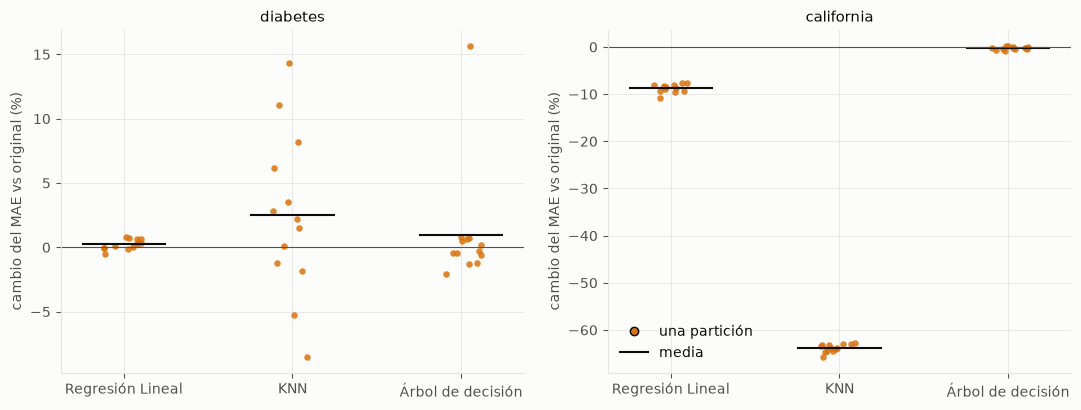
\includegraphics[width=\textwidth]{img/cambio_mae_particiones.png}
\caption{Cambio del MAE al aplicar la transformación aprendida, respecto a los atributos originales, en cada una de las 13 particiones. Cada punto es una partición y la línea negra, la media. Valores negativos indican mejora.}
\label{fig:cambio-mae-particiones}
\end{figure}

En Diabetes la media de KNN esconde una dispersión enorme que va desde un -8\% a un 14\%. Esto no necesariamente quiere decir que la transformación empeore de forma consistente, sino que es inestable para este dataset. Con tan pocos datos, la métrica aprendida acaba sobreajustándose en unas particiones, mientras que consigue acertar en otras. 

Pasando al árbol de decisión en Diabetes, hay un punto en 15\% que tira de la media hacia arriba, el resto se reparte en torno a cero. Es coherente con el valor de p=0.89, porque el test de rangos no se deja arrastrar por un valor extremo tanto como la media. En California el cambio es prácticamente nulo, lo cual tiene sentido dado que los árboles son invariantes a transformaciones monótonas por atributo; una métrica que reescala atributos apenas les afecta. 

Con estos resultados nos preguntamos si realmente importa el algorirmo evolutivo, qué ocurre en otros datasets y si se puede mejorar la representación o la regla de predicción. 

\subsection{Los datasets}
Antes de generalizar, tenemos que ver con qué clase de datos estamos trabajando. La \autoref{tab:datasets} muestra el número de muestras y de atributos de cada dataset (después de habernos quedado solo con los atributos numéricos y de limitar a 10.000 filas).

\begin{table}[h]
\centering
\begin{tabular}{lrrl}
\hline
\textbf{Dataset} & \textbf{Muestras} & \textbf{Atributos} & \textbf{Origen} \\
\hline
diabetes                                 & 442        & 10 & práctica \\
california                               & 20\,640    & 8  & práctica \\
\hline
concrete\_compressive\_strength          & 1\,030     & 8  & OpenML \\
stock                                    & 950        & 9  & OpenML \\
space\_ga                                & 3\,107     & 6  & OpenML \\
sulfur                                   & 10\,000    & 6  & OpenML \\
kin8nm                                   & 8\,192     & 8  & OpenML \\
bank8FM                                  & 8\,192     & 8  & OpenML \\
puma8NH                                  & 8\,192     & 8  & OpenML \\
house\_8L                                & 10\,000    & 8  & OpenML \\
cpu\_small                               & 8\,192     & 12 & OpenML \\
wine\_quality                            & 6\,497     & 11 & OpenML \\
\hline
\end{tabular}
\caption{Conjuntos de datos utilizados: los dos de la práctica y diez de regresión adicionales de OpenML.}
\label{tab:datasets}
\end{table}

Como se puede observar, son datasets pequeños o medianos, con entre 6 y 12 atributos numéricos. Los hemos escogido principalmente porque estaban diseñados para tareas de regresión, por su tamaño manejable y por su disponibilidad en OpenML. 

\subsection{Comparación con otras técnicas bioinspiradas e importancia del algoritmo evolutivo.}

En el paper de referencia se clasifican los algoritmos evolutivos en cuatro familias: enjambres, bioinspirados no basados en enjambre, físicos y químicos. Quisimos averiguar si había otra técnica mejor que CMA-ES para este problema. 

\subsubsection{Diseño del test}
\begin{itemize}
    \item Los mismo 20 y 16 parámetros ($\theta$), el mismo fitness (media de regresión lineal y KNN como en el notebook principal) y el mismo presupuesto de 1.000 evaluaciones para todos. 
    \item 20 algoritmos, casi todos de la primera tabla del paper, usando la librería \texttt{mealpy}, un algoritmo genético propio, CMA-ES, una búsqueda aleatoria y el punto inicial sin búsqueda. 
    \item El punto inicial $\theta_0$ se incluye en la población de partida de todos para que ninguno parta con desventaja. 
    \item Dos particiones por dataset - test rápido de carácter exploratorio.
\end{itemize}

Hay que tener cuidado porque algoritmos como BFO, CSO, CSA y FFA gastan muchas evaluaciones por iteración. Con 1000 evaluaciones, apenas consiguen completar una generación, por lo que sus resultados son básicamente los de elegir el mejor de unos 30 puntos aleatorios. No sacaremos conclusiones sobre ellos. En la \autoref{tab:rango-algoritmos} podemos ver el rango medio de cada algoritmo según el fitness alcanzado. 

\begin{table}[h]
\centering
\begin{tabular}{lr}
\hline
\textbf{Algoritmo} & \textbf{Rango medio} \\
\hline
CMA-ES             & $2.0$ \\
GA (propio)        & $2.5$ \\
BBO (biogeografía) & $3.5$ \\
HS (armonía)       & $3.5$ \\
DE                 & $4.5$ \\
ICA (imperialista) & $6.5$ \\
ACOR               & $7.5$ \\
ABC                & $7.5$ \\
\hline
\end{tabular}
\caption{Rango medio de cada algoritmo según el fitness alcanzado (1 = mejor).}
\label{tab:rango-algoritmos}
\end{table}

En la \autoref{fig:comparativa-algoritmos}, la barra es la media del cambio del MAE de validación (promedio de regresión lineal y KNN) en las dos particiones. Las barras hacia la izquierda se pueden interpretar como mejoras. Lo que hay que comparar, no obstante, es la diferencia entre los algoritmos, y hay que mirarla en relación a la que hay entre el punto inicial sin búsqueda, y la búsquea aleatoria (barras azules), que es lo que se consigue ''sin esfuerzo''. 

\begin{figure}[h]
\centering
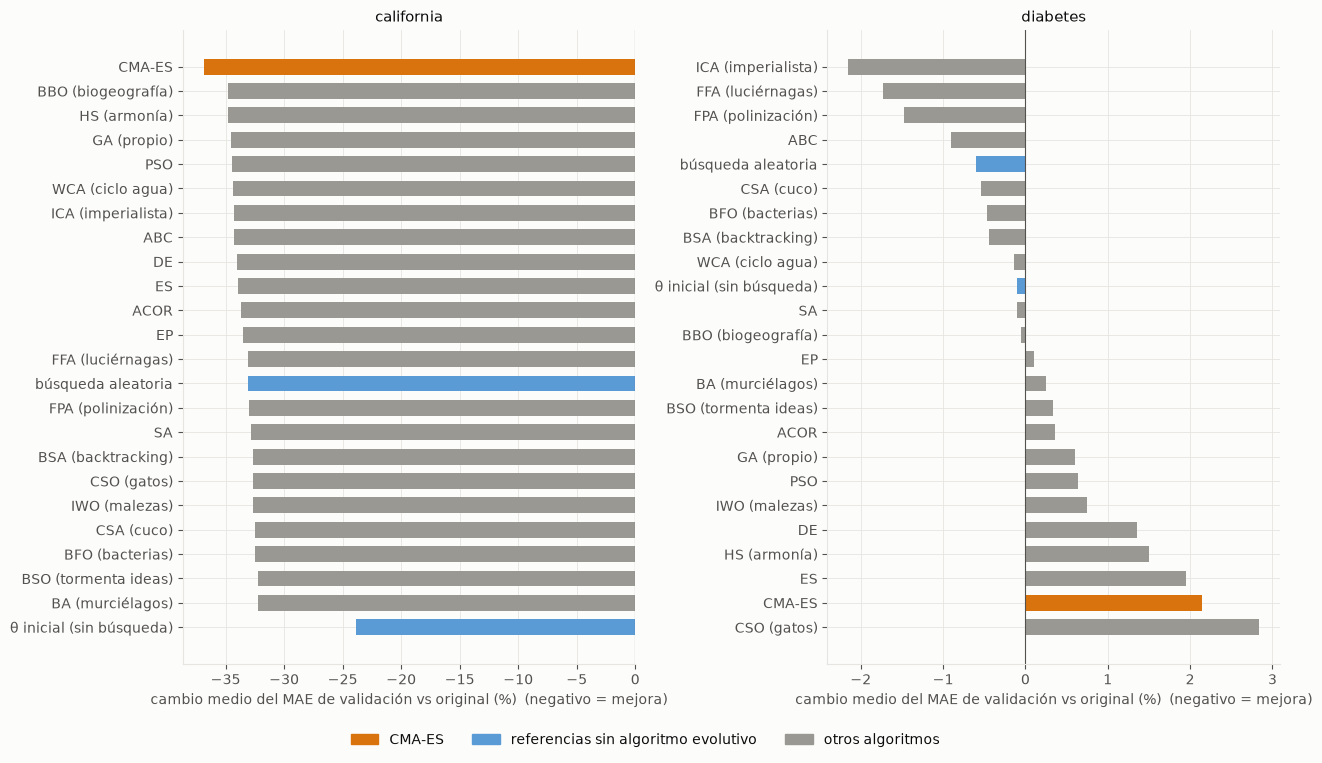
\includegraphics[width=\textwidth]{img/comparativa_algoritmos.png}
\caption{Cambio medio del MAE de validación respecto a los atributos originales para cada algoritmo de optimización. En naranja, CMA-ES; en azul, las referencias sin algoritmo evolutivo (parámetros iniciales y búsqueda aleatoria). Valores negativos indican mejora.}
\label{fig:comparativa-algoritmos}
\end{figure}

Podemos ver que en California casi todos los algoritmos consiguen entre un 32\% y un 37\% de mejora. Incluso la búsqueda aleatoria logra un 33\%. CMA-ES es el primero por poco, siendo la distancia entre los mejores algoritmos de 2-3 puntos con solo dos particiones. Por ello esto debe cogerse por pinzas y no es concluyente. Lo que importa es la familia de transformaciones, no el algoritmo que la busca.

En Diabetes ningún algoritmo mejora de forma fiable, las barras van de -2\% a 3\% y además tienen mucho ruido. CMA-ES sigue tenienod el mejor fitness, pero en validación empeora KNN. El cuello de botella, por ende, no es la potencia de búsqueda. 

Nos quedamos con CMA-ES porque tiene el mejor rango medio por fitness (2.0 seguido de cerca por el GA propio con 2.5). Es de los más baratos en tiempo y está justificado teóricamente para este tipo de porblemas continuo, sin gradiente y no separable. No es la única opción razonable, pero es la que se ha escogido. 

\subsection{¿Se puede mejorar CMA-ES con un híbrido?}
Como Diabetes fallaba por sobreajuste al fitness, probamos a diseñar un algoritmo nuevo que mezclara lo mejor de varios, partiendo del CMA-ES y probando cuatro modificaciones, cada una pensada para un problema concreto. Estas modificaciones quedan descritas en la \autoref{tab:variantes-hibridas} Además todas se evalúan con 1.000 evaluaciones y 5 particiones por dataset. 

\begin{table}[h]
\centering
\begin{tabular}{p{2.6cm}p{6.8cm}p{3.6cm}}
\hline
\textbf{Variante} & \textbf{Qué añade} & \textbf{Para qué} \\
\hline
CMA+folds & Cambia los pliegues de validación cruzada en cada generación (el fitness pasa a ser estocástico) & Que la búsqueda no se ajuste a unos pliegues concretos \\
\hline
CMA+DE & Inyecta en cada generación un individuo de cruce diferencial (de evolución diferencial) & Más diversidad, algo propio de DE y los algoritmos genéticos \\
\hline
CMA+folds+sel & Lo primero más una selección final: reservamos 100 evaluaciones para puntuar los mejores candidatos en pliegues nuevos, y solo aceptamos el aprendido si mejora a $\theta_0$ en más de $0.005$ & Elegir de forma robusta \\
\hline
Híbrido completo & Pliegues cambiantes, DE y selección final & Todo junto \\
\hline
\end{tabular}
\caption{Variantes híbridas de CMA-ES evaluadas.}
\label{tab:variantes-hibridas}
\end{table}

En la \autoref{tab:resultados-hibridos} podemos ver la diferenci amedia del cambio del MAE (puntos porcentuales) entre cada una de las variantes respecto al CMA-ES base, sobre 6 particiones. Valores positivos nos indican que la variante ha empeorado sus resultados. La columna ''Mejor que base'' cuenta cuántas de las particiones han conseguido mejorar a CMA-ES. 

\begin{table}[h]
\centering
\begin{tabular}{llrcr}
\hline
\textbf{Dataset} & \textbf{Variante} & \textbf{Dif. media (p.p.)} & \textbf{Mejor que base} & $\boldsymbol{p}$ \textbf{(Wilcoxon)} \\
\hline
california & CMA+folds              & $+7.09$ & 0/6 & $0.031$ \\
           & CMA+DE                 & $-0.28$ & 4/6 & $0.562$ \\
           & CMA+folds+sel          & $+0.40$ & 3/6 & $0.562$ \\
           & Híbrido (folds+DE+sel) & $+0.30$ & 2/6 & $0.688$ \\
\hline
diabetes   & CMA+folds              & $+1.24$ & 3/6 & $0.688$ \\
           & CMA+DE                 & $+1.53$ & 3/6 & $0.438$ \\
           & CMA+folds+sel          & $+0.98$ & 1/6 & $0.312$ \\
           & Híbrido (folds+DE+sel) & $+1.57$ & 0/6 & $0.031$ \\
\hline
\end{tabular}
\caption{Diferencia media, en puntos porcentuales de cambio del MAE, entre cada variante y CMA-ES base, sobre 6 particiones. Valores positivos indican que la variante es peor. \emph{Mejor que base} cuenta las particiones en que la variante mejora a CMA-ES.}
\label{tab:resultados-hibridos}
\end{table}

Adicionalmente, la \autoref{fig:variantes-hibridas} nos muestra de manera visual este cambio medio del MAE. Las barras representan la media en 6 particiones, mientras que la línea vertical sobre ellas representa la desviación típica entre las particiones. Si las líneas de dos variantes se solapan demasiado, la diferencia entre ellas pasa a no ser fiable. 

\begin{figure}[h]
\centering
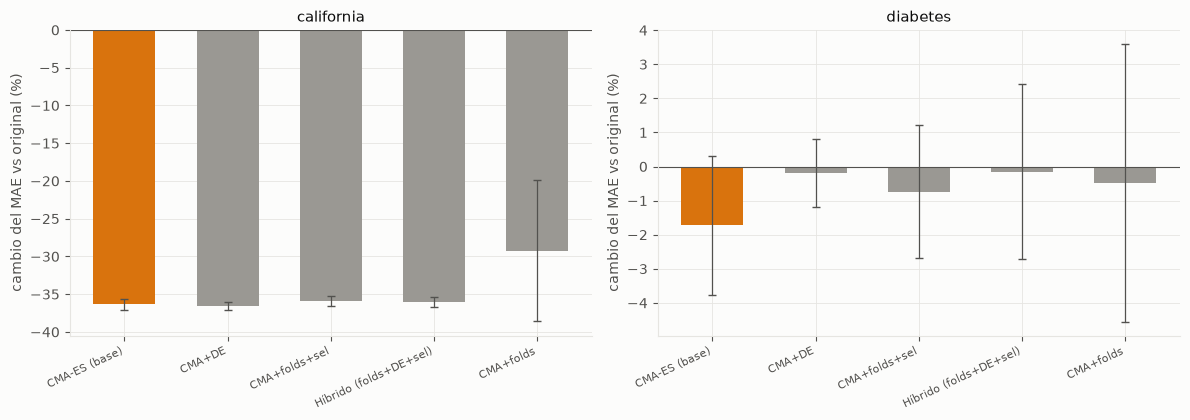
\includegraphics[width=0.8\textwidth]{img/variantes_hibridas.png}
\caption{Cambio medio del MAE respecto a los atributos originales para CMA-ES base (en naranja) y sus variantes híbridas, sobre 6 particiones. Las barras de error indican la desviación típica entre particiones. Valores negativos indican mejora.}
\label{fig:variantes-hibridas}
\end{figure}

Vemos que ninguna variante mejora al CMA-ES base. En California, DE y la selección robusta no cambian nada: tenemos diferencias de décimas de punto. En Diabetes ninguna mejora y el híbrido completo es peor en las seis particiones. Además, los pliegues cambiantes empeoran de manera clara en California. Unos siete puntos porcentuales peor, con una dispersión entre las particiones casi trece veces mayor. Esto puede deberse a que en cada generación se están comparando a candidatos con un ruido distinto y CMA-ES --- que se apoya en ordenar bien a los candidatos de una generación --- avanza peor. Nuestra hipótesis era que este híbrido conseguiría reducir el sobreajuste en Diabetes, pero no hemos podido confirmarlo. 

Lo que aprendemos de esta sección es que inventar un algoritmo nuevo no tenía sentido en este punto. Lo que mueve los resultados son la representación y la regla de predicción, no la búsqueda en sí. Por ello, el resto de experimentos los centraremos en esto. 

\subsection{Introducción de PCA dentro de la búsqueda para la reducción de ruido. }

La idea es que la propia búsqueda decida qué componentes principales conservar, como un método alternativo de reducir el ruido. La representación pasaría a ser: 
\begin{enumerate}
    \item Yeo-Johnson 
    \item Estandarización 
    \item Pesos por atributo 
    \item PCA
    \item Pesos por componente
\end{enumerate}

Con todos los pesos en 1 es una rotación, y las distancias son idénticas a las de la estandarización,  por lo que la búsqueda también arranca de la línea base. El peso de cada componente lo aprende CMA-ES: un peso cercano a 0 equivale a descartar ese componente (reducción de ruido aprendido). Añade $n$ parámetros ($3n$ en total). Probamos también una variante con solo dos parámetros --- un corte y una suavidad --- y la comparamos con el PCA clásico que conserva el 95\% de la varianza.

El diseño lo hacemos en dos fases para evitar el sesgo de selección. Una primera tanda con semillas del 13 al 15 se usan para elegir la variante, y una tanda de confirmación con 10 particiones nuevas (semillas de 30 a 39) que permite decidir antes de mirar que el PCA solo entraría en el método final si mejoraba de forma consistente. Las siguientes gráficas usan la tanda de confirmación. En la \autoref{tab:comparativa-pca} vemos que la versión con PCA mejora solo en un 0.003, una diferencia no significativa. Esto nos puede indicar que una rotación de los ejes no aporta nada sobre reescalar los atributos originales.

\begin{table}[h]
\centering
\begin{tabular}{lr}
\hline
\textbf{Transformación} & \textbf{KNN} \\
\hline
Crudo                              & $1.000$ \\
Estándar                           & $0.871$ \\
CMA-ES (YJ + pesos)                & $0.748$ \\
CMA-ES + PCA (peso por componente) & $0.745$ \\
\hline
\end{tabular}
\caption{MAE de KNN con cada transformación, relativo al obtenido con los atributos originales (crudo = 1).}
\label{tab:comparativa-pca}
\end{table}

\begin{figure}[h]
\centering
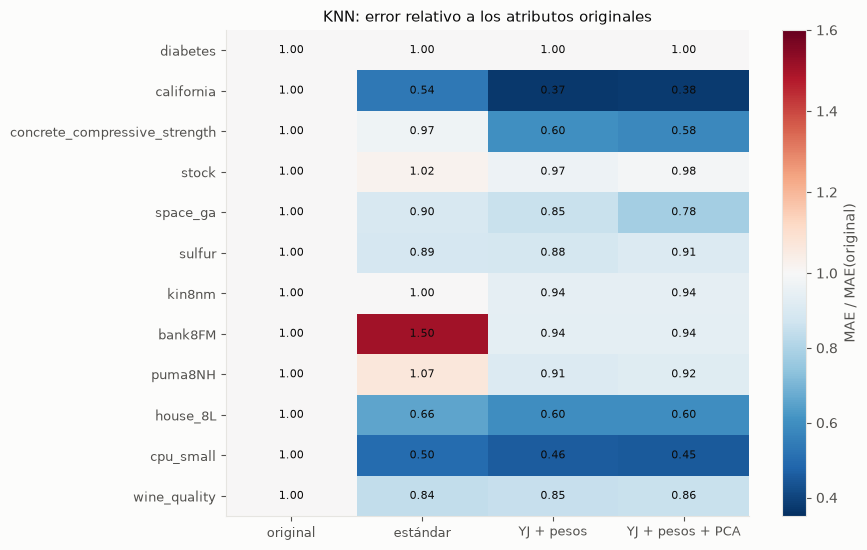
\includegraphics[width=0.85\textwidth]{img/heatmap_knn_datasets.png}
\caption{MAE de KNN con cada transformación, relativo al obtenido con los atributos originales, en los 12 datasets. Azul indica mejora (valor menor que 1) y rojo, empeoramiento.}
\label{fig:heatmap-knn}
\end{figure}

En la \autoref{fig:heatmap-knn} vemos un mapa de calor donde cada celda es el cociente entre el error de ese método y el del dataset con los atributos originales. Los valores son, por ende, la media geométrica de las columnas. Por debajo de 1 (azul) se mejora, y por encima del 1 (naranja) empeora. Una columna de azules uniformes nos indica que el método funciona por lo general, mientras que una fila de naranjas indica un dataset difícil. 

Se observa que estandarizar solo mejora en unos datasets y empeora en otros --- por ejemplo el de banca, donde ya parte de un putno mucho peor que los datos originales. La columna de ''YJ + pesos'' es mucho más azul que ''estándar'', mejorando en 11/12 datasets. Además, concluimos que añadir el PCA apenas cambia la columna, ya que se ve casi igual que la de ''YJ + pesos''. De hecho, en la \autoref{fig:efecto-pca} podemos ver el cambio medio del error al añadir PCA por dataset (barras). Un asterisco indica que ese cambio es estadísticamente distinguible de cero con 10 particiones. Si las barras se reparten a ambos lados, el efecto medio se anula; y esto es lo que observamos en la mayoría de casos.

\begin{figure}[h]
\centering
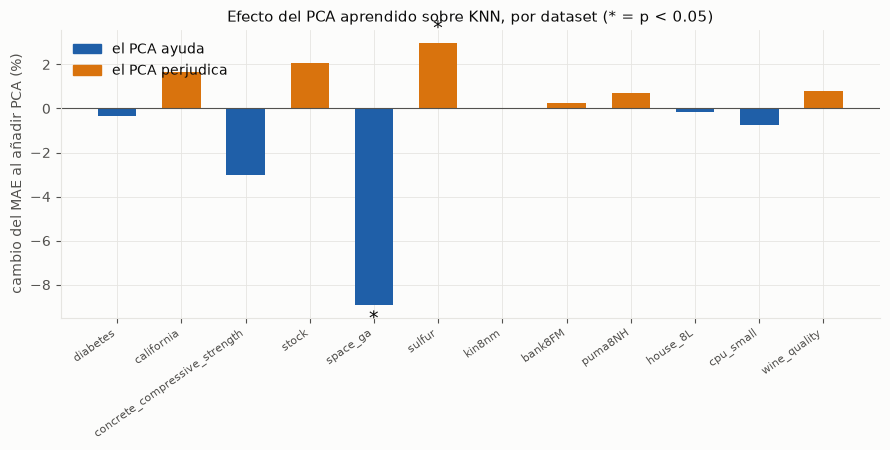
\includegraphics[width=0.75\textwidth]{img/efecto_pca_knn.png}
\caption{Cambio del MAE de KNN al añadir la rotación PCA a la transformación aprendida (YJ + pesos), por dataset. En azul, los datasets donde PCA mejora; en naranja, donde empeora. El asterisco marca diferencias significativas ($p < 0.05$, test de Wilcoxon).}
\label{fig:efecto-pca}
\end{figure}

Se observa que en conjunto, el PCA apenas aporta nada. El cambio global es de apenas un -0.4\% y el p-valor se acerca a 1. Con el criterio fijado, el PCA queda por fuera del método final. Aunque eso no quiere decir que no ayude en todos los datasets, de hecho, aporta bastante en \texttt{space\_ga} (alrededor de un 9\% menos de error, mejorando en todas las particiones). Esto puede deberse a que los atributos ya estaban de partida muy correlacionados, que es donde rotar puede tener sentido. Sin embargo, perjudica a otros datasets como \texttt{sulfur} y \texttt{stock}. 

El PCA clásico con el corte en el 95\% de varianza empeora la estandarización en la primera tanda --- 0.896 frente a 0.873 de media --- por lo que quitar componentes de forma fija no parece ser la mejor forma de reducir el ruido. 

En la primera tanda de 3 particiones el PCA parecía mejorar en los 12 datasets, pero cuando lo intentamos confirmar con más particiones nuevas la ventaja despaarece. Por eso insistimos en usar particiones que no se usaron para elegir a la hora de evaluar si los cambios en el método son significativos. 

\subsection{Cambiar la regla de predicción: regresión lineal local.}
Como lo que mueve los resultados es la regla de predicción y no el algoritmo evolutivo, vamos a probar con una regla local lineal. El experimento separa dos preguntas con cinco configuraciones: 6 particiones nuevas en cada uno de los 12 datasets. Estas preguntas y configuraciones se recogen en la \autoref{tab:comparaciones}.

\begin{table}[h]
\centering
\begin{tabular}{p{5.5cm}p{7.5cm}}
\hline
\textbf{Configuración} & \textbf{Qué responde} \\
\hline
estándar + KNN y estándar + LLR & ¿Ayuda la regla por sí sola, sin aprender nada? \\
\hline
métrica(KNN) + KNN y métrica(KNN) + LLR & Con la misma métrica, ¿ayuda cambiar la regla? \\
\hline
métrica(LLR) + LLR & ¿Ayuda optimizar la métrica directamente para la regla? \\
\hline
\end{tabular}
\caption{Comparaciones planteadas entre configuraciones y la pregunta que responde cada una.}
\label{tab:comparaciones}
\end{table}

En las cuatro primeras $k$ y el ridge se eligen por validación cruzada en una rejilla de 15 combinaciones. En la última los aprende CMA-ES junto con la métrica. Esa última configuración es el método completo. 

En la \autoref{tab:resultados-llr} podemos ver el MAE de cada configuración en relación al de KNN con los atributos originales. Con esto podemos responder a las tres preguntas de la tabla anterior. En primer lugar, que la regla de por sí ayuda, ya que el paso de KNN a LLR con atributos estandarizados --- 0.840 a 0.737 --- da casi lo mismo que aprender la métrica para KNN (0.724) sin optimizar nada. Además, con la misma métrica, vemos que cambiar la regla ayuda, pasando de un 0.724 a un 0.673 en meida (geométrica). Finalmente, también comprobamos que ayuda optimizar la métrica para la regla, aunque la ganancia es más pequeña.

\begin{table}[h]
\centering
\begin{tabular}{lr}
\hline
\textbf{Configuración} & \textbf{MAE relativo} \\
\hline
estándar + KNN      & $0.840$ \\
estándar + LLR      & $0.737$ \\
métrica(KNN) + KNN  & $0.724$ \\
métrica(KNN) + LLR  & $0.673$ \\
métrica(LLR) + LLR  & $\mathbf{0.641}$ \\
\hline
\end{tabular}
\caption{MAE de cada configuración relativo al de KNN con los atributos originales (media geométrica sobre los 12 datasets). Menor es mejor.}
\label{tab:resultados-llr}
\end{table}

En la \autoref{fig:resultados-llr}, la gráfica de la izquierda muestra la media geométrica del cociente entre el error de cada método y el de KNN con los atributos originales (a menor valor, mejor). El mapa de color de la derecha desglosa dicho cociente por dataset. En la \autoref{tab:contrastes-llr}, \emph{Cambio} es la variación media del error entre los dos métodos que se comparan; \emph{Mejor en} cuenta en cuántos de los 72 casos gana el primero, y $p$ es el p-valor del test de Wilcoxon por pares.

\begin{figure}[h]
\centering
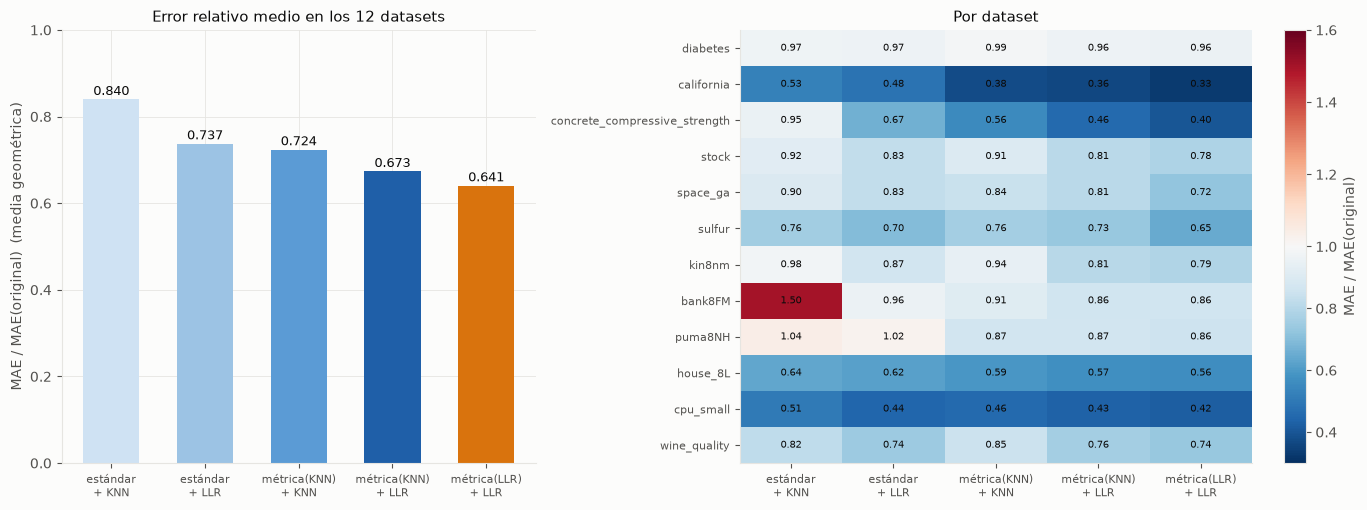
\includegraphics[width=\textwidth]{img/resultados_llr.png}
\caption{Izquierda: MAE relativo a KNN con los atributos originales, como media geométrica sobre los 12 datasets; en naranja, el método completo. Derecha: el mismo cociente por dataset. Azul indica mejora (valor menor que 1) y rojo, empeoramiento.}
\label{fig:resultados-llr}
\end{figure}

Vemos que cada paso mejora al anterior, la media geométrica baja de 0.84 (estándar + KNN) a 0.64 (método completo). Frente a los datos originales, obtenemos un 36\% menos de error. Además, vemos también que la regla local lineal ayuda por sí sola, ya que con datos estándar baja el error un 12\% respecto a KNN, ganando en 68 de 72 parejas. Una parte de la mejora del método completo viene de usar una regla más flexible, y no tanto de la métrica. Frente a la regla local sin aprender, el método completo baja el error un 13\%, y optimizar la métrica para la regla gana casi un 5\% a reutilizar la métrica de KNN con la regla local lineal. Es un cambio pequeño, pero consistente, ganando en 56 de 72 parejas. 

Adicionalmente, es consistente entre datasets. El método completo está por debajo de 1 en los 12 datasets. Las mayores mejoras llegan la 60-67\% de reducción del error, siendo el menor \texttt{diabetes}, donde solo llega a un 4\%. 

Algunas cosas a tener en cuenta son: primero, que la última configuración aprende \textit{k} y el ridge con 1000 evaluaciones de CMA-ES, mientras que las demás los eligen en una rejilla de 15 combinaciones. Parte de la ventaja puede ser simplemente más ajuste de hiperparámetros. Segundo, tarda mucho más.

\begin{table}[h]
\centering
\begin{tabular}{p{7cm}rcr}
\hline
\textbf{Comparación} & \textbf{Cambio} & \textbf{Mejor en} & $\boldsymbol{p}$ \textbf{(Wilcoxon)} \\
\hline
estándar + LLR frente a estándar + KNN \newline {\small (la regla sola)}                 & $-12.1$\,\% & 68/72 & $<0.0001$ \\
métrica(KNN) + LLR frente a métrica(KNN) + KNN \newline {\small (cambiar la regla)}       & $-6.9$\,\%  & 67/72 & $<0.0001$ \\
métrica(LLR) + LLR frente a métrica(KNN) + LLR \newline {\small (optimizar para la regla)} & $-4.9$\,\%  & 56/72 & $<0.0001$ \\
\hline
métrica(LLR) + LLR frente a estándar + LLR                                               & $-13.2$\,\% & 66/72 & $<0.0001$ \\
métrica(LLR) + LLR frente a estándar + KNN                                               & $-23.7$\,\% & 69/72 & $<0.0001$ \\
\hline
\end{tabular}
\caption{Contrastes entre configuraciones sobre 72 casos (12 datasets $\times$ 6 particiones). \emph{Cambio} es la variación media del MAE de la primera configuración respecto a la segunda; \emph{Mejor en} cuenta los casos en que la primera tiene menor error.}
\label{tab:contrastes-llr}
\end{table}

\subsection{¿Cómo queda frente a otros modelos a nivel absoluto?}
Que un método mejore a KNN no dice si es bueno en términos absolutos. Lo comparamos con los modelos que suelen ganar en datos tabulares: 

\begin{itemize}
    \item Random Forest con 200 árboles y Gradient Boosting (\texttt{HistGradientBoosting}) ajustados con una búsqueda aleatoria de 30 configuraciones y validación cruzada de 3 pliegues y reentrenados con todo el entrenamiento. 
    \item Proceso gaussiano con ARD --- una esclaa por atributo, estimada por máxima verosimilitud. Es el competidor teórico más cercano porque aprende justo lo que aprendemos nosotros, pesos por atributo. Lo entrenamos con una submuestra de 2000 filas por coste, lo que le da menos datos que a nuestro método. 
\end{itemize}

\begin{figure}[h]
\centering
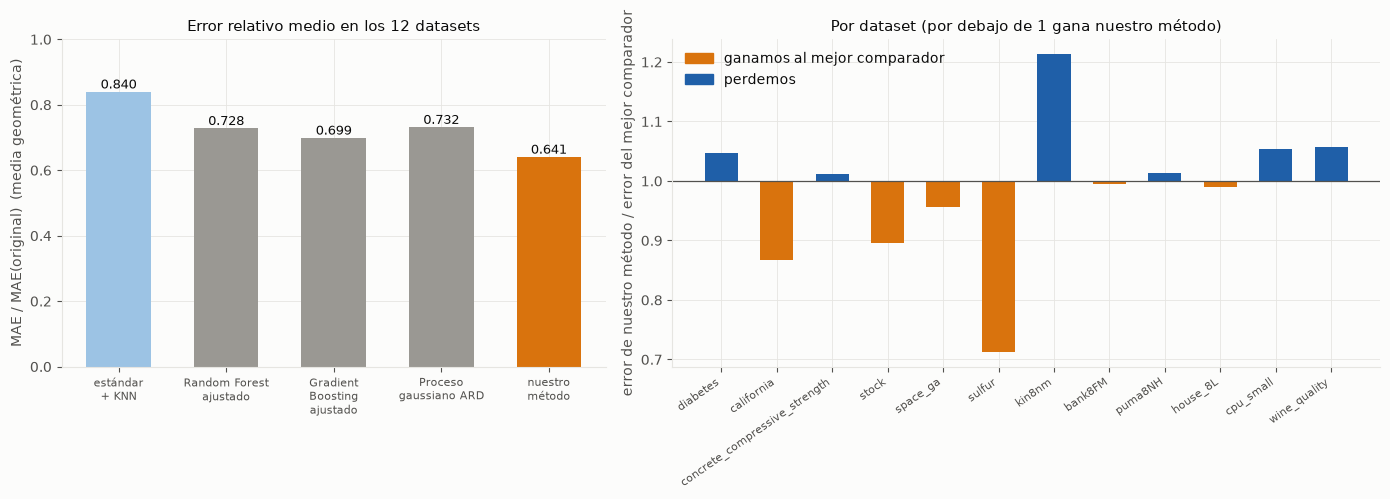
\includegraphics[width=\textwidth]{img/comparativa_modelos.png}
\caption{Izquierda: MAE relativo a KNN con los atributos originales (media geométrica sobre los 12 datasets) de nuestro método frente a otros modelos de regresión. Derecha: cociente entre el error de nuestro método y el del mejor de los comparadores en cada dataset; por debajo de 1, nuestro método gana.}
\label{fig:comparativa-modelos}
\end{figure}

En la \autoref{fig:comparativa-modelos}, a la izquierda nos fijamos en los errores relativos, a menor valor, mejor. Y a la derecha, cada barra representa el cociente entre el error de nuestro método y el del mejor de los tres comparadores del dataset: por debajo de 1 (naranja) ganamos, y por encima (azul), perdemos. Este cociente es una comparación dura, porque el mejor comparador se elige después de ver los resultados\dots

Vemos que de media nuestro método tiene el menor error, y frente a cada uno por separado la ventaja es del 8\% al 12\% y significativa (p de Wilcoxon). Además, frente al mejor de los tres en cada pareja, la diferencia es de aproximadamente un -2\%, lo cual en este caso no es significativo. Es decir, que estamos a la altura del mejor modelo de referencia, pero no por encima. Finalmente, por dataset hay ganadores distintos, por lo que el resultado también depende en gran medida de la naturaleza de los datos y atributos del problema.

\begin{table}[h]
\centering
\begin{tabular}{p{7cm}rcr}
\hline
\textbf{Comparación} & \textbf{Cambio} & \textbf{Mejor en} & $\boldsymbol{p}$ \textbf{(Wilcoxon)} \\
\hline
Nuestro método frente a Random Forest ajustado      & $-12.0$\,\% & 58/72 & $<0.0001$ \\
Nuestro método frente a Gradient Boosting ajustado  & $-8.3$\,\%  & 53/72 & $<0.0001$ \\
Nuestro método frente a proceso gaussiano ARD       & $-12.4$\,\% & 51/72 & $<0.0001$ \\
\hline
Nuestro método frente al mejor de los tres en cada dataset & $-2.1$\,\% & 33/72 & $0.618$ \\
\hline
\end{tabular}
\caption{Contrastes entre nuestro método y otros modelos de regresión sobre 72 casos (12 datasets $\times$ 6 particiones). \emph{Cambio} es la variación media del MAE de nuestro método respecto al comparador; \emph{Mejor en} cuenta los casos en que nuestro método tiene menor error.}
\label{tab:contrastes-modelos}
\end{table}

En la \autoref{tab:contrastes-modelos} podemos ver los contrastes entre nuestro modelo y los otros sobre los 72 casos. La última fila es la más interesante, ya que muestra que ganamos en menos de la mitad de los casos, pero con un cambio medio negativo de -2.1\%. Esto es interesante, porque cuando ganamso lo hacemos por más margen que cuando perdemos. No obstante, con un $p=0.618$ no hay diferencia significativa. Volvemos a la conclusión de que nuestro método está a la par del mejor modelo elegido a posteriori en cada dataset, y supera de forma significativa a cada uno de ellos por separado. 

Sin embargo, otro punto a tener en cuenta es que el proceso gaussiano solo ve 2000 filas, lo que perjudica en los datasets grandes. Nuestro método ajusta más hiperparámetros (exponentes, peso, k, ridge) que Random Forest y Gradient Boosting, que solo ajustan 30 configuraciones aleatorias. 

\subsection{Caso de Diabetes}
Diabetes es el único dataset de la práctica donde el método no cumple el criterio de $e' < e$, y necesitamos saber por qué. Mostramos el cambio del error por partición para los cuatro métodos de la confirmación en 10 particiones.

\begin{figure}[h]
\centering
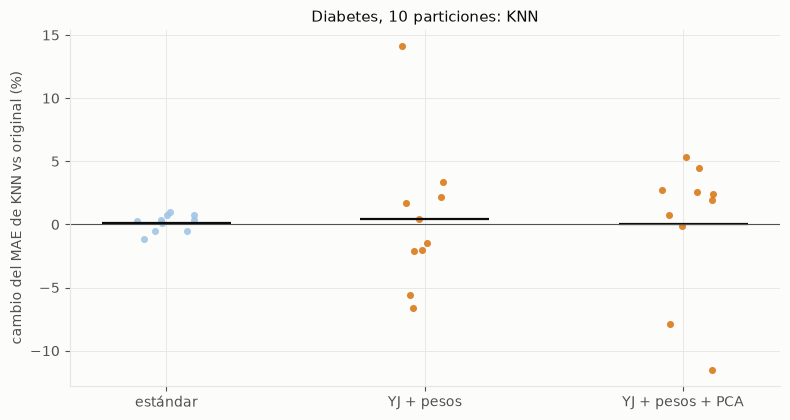
\includegraphics[width=0.7\textwidth]{img/diabetes_particiones_knn.png}
\caption{Cambio del MAE de KNN respecto a los atributos originales en diabetes, para cada una de las 10 particiones. Cada punto es una partición y la línea negra, la media.}
\label{fig:diabetes-particiones}
\end{figure}

\begin{table}[h]
\centering
\begin{tabular}{lrr}
\hline
\textbf{Transformación} & \textbf{Media} & \textbf{Desviación típica} \\
\hline
Estándar                                & $+0.13$\,\% & $0.66$ \\
CMA-ES (YJ + pesos)                     & $+0.40$\,\% & $5.80$ \\
CMA-ES + PCA (peso por componente)      & $+0.07$\,\% & $5.45$ \\
\hline
\end{tabular}
\caption{Media y desviación típica, sobre 10 particiones, del cambio del MAE de KNN respecto a los atributos originales en diabetes.}
\label{tab:diabetes-dispersion}
\end{table}

En la \autoref{fig:diabetes-particiones} vemos que los puntos están repartidos a ambos lados de cero, por lo que no podemos demostrar que haya una mejora. En la \autoref{tab:diabetes-dispersion} se recogen la media y la desviación típica sorbe las 10 particiones, respecto al cambio del MAE de KNN respecto a los atributos originales en diabetes. 

Con 10 particiones nuevas, el cambio medio es prácticamente nulo para todos los métodos, con una desviación de unos 5-6 puntos porcentuales entre particiones. Por ende, la conclusión es que no hay mejora en Diabetes. Esto se puede deber a la poca presencia de datos, con solo 309 muestras de entrenamiento para ajustar 20 parámetros con un fitness que usa validación cruzada sobre esas mismas muestras. La búsqueda mejora el fitness --- bajada de 5-8\% --- pero esa mejora no llega a trasladarse a validación: sobreajuste al criterio de búsqueda\dots

Probamos regularizar hacia $\theta_0$, usar un único exponente compartido, pliegues cambiantes y selección robusta con validación independiente; pero ninguna mejora Diabetes de forma consistente. Los propios datos explican que el margen sea bajo, ya que los datos ya vienen centralizados y escalas parecidas, por lo que estandarizar no cambia nada y tampoco hay colas largas que requieran de corrección. 

En una tanda con solo 2 particiones, CMA-ES sale con +2.2\% en Diabetes, y con 6 particiones con -1.7\% (en ambos casos, promedio de regresión lineal y KNN).El signo cambiaba con el número de particiones. Con una desviación de 5-6 puntos. Por ende, podemos concluir que cualquier interpretación sobre Diabetes con pocas particiones se basa en ruido.
\newpage
\section{Análisis global}
\subsection{Qué hemos aprendido en orden}

En la \autoref{tab:resumen} se resumen las respuestas a las preguntas que se han ido formulando durante el desarrollo del trabajo. 

\begin{table}[h]
\centering
\begin{tabular}{p{5.2cm}p{6.3cm}p{1.8cm}}
\hline
\textbf{Pregunta} & \textbf{Respuesta} & \textbf{Evidencia} \\
\hline
¿Funciona aprender la transformación con CMA-ES? & Sí, y mucho en California; no en Diabetes & 5.0 (13 particiones) \\
\hline
¿Importa qué algoritmo evolutivo se use? & Poco; CMA-ES es la opción más razonable & 5.2 \\
\hline
¿Mejora un híbrido a CMA-ES (pliegues cambiantes, DE, selección)? & No & 5.3 \\
\hline
¿Ayuda el PCA dentro de la búsqueda? & No de forma consistente (sí en \texttt{space\_ga}, no en \texttt{sulfur}) & 5.4 \\
\hline
¿Generaliza a otros datasets? & Sí: KNN mejora un 25\,\% de media (11 de 12 datasets) & 5.4 \\
\hline
¿Ayuda una regla local lineal y optimizar la métrica para ella? & Sí: otro 13\,\% frente a esa regla sin aprender & 5.5 \\
\hline
¿Es competitivo con modelos de referencia? & Sí, a la altura del mejor de ellos, no por encima & 5.6 \\
\hline
¿Y en Diabetes? & No mejora; sobreajuste por pocos datos & 5.7 \\
\hline
\end{tabular}
\caption{Resumen de las preguntas planteadas y de la sección donde se encuentra la evidencia de cada respuesta.}
\label{tab:resumen}
\end{table}

\subsection{Qué podemos afirmar}
\begin{itemize}
    \item Una transformaciín por atributo --- exponente de Yeo-Johnson y peso --- aprendida con CMA-ES mejora de forma sustancial a todos los modelos basados en distancias. Con 10 particiones nuevas y 12 datasets, KNN reduce su error un 25\% respecto a los atributos originales, y 14\% respecto a la estandarización simple. Con regresión linela, la mejora es del 6-7\% y con el árbol de decisión nula, como se espera por su invarianza. 
    \item La mejora cumple el criterio del enunciado de $e'<e$ en la gran mayoría de datasets para KNN y en la mayoría para regresión lineal. Sin embargo, no llega a cumplirlo en Diabetes. 
    \item Cambiar la regla de predicción a regresión lineal local y optimizar la métrica para ella da una mejora adicional respecto a usar la métrica de KNN. Es un efecto pequeño pero consistente. 
    \item El método es competitivo con Random Forest, Gradient Boosting y procesos gaussianos ARD ajustados. Su error medio es menor que el de cada uno por separado, y comparable al del mejor de ellos en cada caso. 
\end{itemize}

\subsection{Lo que no podemos afirmar}
\begin{itemize}
    \item Aprender métricas para KNN, ponderar atributos con CMA-ES y la regresión lineal local están publicados. Lo que no hemos encontrado publicado es la combinación concreta, pero nuestra búsqueda bibliográfica puede estar limitada. 
    \item Tampoco podemos confirmar que el algoritmo evolutivo sea lo que produce la mejora. La búsqueda aleatoria con el mimso presupuesto ya consigue la mayor parte en California. Lo que importa es la familia de transformaciones y la regla de predicción. 
    \item No creemos que supere a modelos de referencia, como mucho estará a su altura con ganadores distintos dependiendo del dataset en el que se aplique. 
    \item Con Diabetes tenemos la hipótesis de que este método no necesariamente tendrá buenos resultados con pocos datos.
\end{itemize}

\subsection{Limitaciones}
En primer lugar, los resultados se basan en doce datasets pequeños o medianos, con atributos numéricos, que han sido elegidos por nosotros. No hay datos con muchas dimensiones, atributos categóricos, valores perdidos o muy ruidosos. Además, se han hecho entre 2 y 13 particiones dependiendo del experimento. Las conclusiones sobre Diabetes necesitan muchas particiones por el ruido y las primeras tandas --- 2 a 3 particiones --- solo son de carácter exploratorio. Por eso confirmamos lo importante con nuevas particiones. 

Nuestro método ajusta más parámetros que modelos de referencia, por lo que parte de la ventaja puede venir de ahí. Además, la búsqueda tarda entre 1-3 minutos por partición, po lo que para un movelo que se entrena una vez es asumible, pero no para un uso interactivo. Finalmente, el fitness depende mucho del modelo objetivo. Optimizamos para KNN o para la regla local lineal, por lo que una trnaformación buena para ellos puede perjudicar a otro modelo. 
\end{document}
